\documentclass[12pt,a4paper]{article}
\usepackage[utf8]{inputenc}
\usepackage{amsmath}
\usepackage{amsfonts}
\usepackage{amssymb}
\usepackage [ngerman] {babel}
\usepackage{hyperref}
\usepackage{array}
\usepackage{longtable}
\usepackage{graphicx}
\usepackage{geometry}


%abstandsformate (z.b. seitenränder)
%\geometry{a4paper, top=25mm, left=33mm, right=22mm, bottom=30mm, headsep=10mm, footskip=12mm}

\begin{document}

\title{Software Engineering Projekt}
\author{Dual Wirtschaftsinformatik Jahrgang 2013 \\ EinkaufsApp}
\date {04. Januar 2015}
\maketitle
\newpage
\tableofcontents
\newpage
\newpage
\section*{Abkürzungsverzeichnis}
\begin{itemize}
\item[1.] EAN - European Article Number
\item[2.] App - Applikation
\item[3.] WG - Wohngemeinschaft
\item[4.] ER - Entity Relationship
\item[5.] UML  - Unified Modeling Language
\item[6.] SSL - Secure Socket Layer 
\item[7.] GTIN - Global Trade Item Number
\end{itemize}
\newpage
\section*{Tabellenverzeichnis}
\begin{itemize}
\item[] Tabelle 1: Anforderungsanalyse
\item[] Tabelle 2 : Ist- Analyse
\item[] Tabelle 3: Meilensteinplanung
\item[] Tabelle 4: Auswertung-Diagramme
\item[] Tabelle 5: Aussichten
\end{itemize}
\newpage
\section*{Abbildungsverzeichnis}
%\addcontentsline{toc}{section}{Abbildungsverzeichnis}
%\listoffigures
\begin{itemize}
\item[] Abbildung 01: Include-Beziehung
\item[] Abbildung 02: Extend-Beziehung
\item[] Abbildung 03: ER - Modell
\item[] Abbildung 04: Aktivitätsliste
\item[] Abbildung 05: Klassen-Diagramm
\item[] Abbildung 06: Flussdiagramm-Login
\item[] Abbildung 07: Marktauswahl
%\item[] Abbildung 08: Aktivitätsdiagramm Einkauf
%HD 01.01.16: wenn wir das von Thomas nehmen dann nur Einzeleinkauf
\item[] Abbildung 08: Einzeleinkauf
\item[] Abbildung 09: Gruppenverwaltung
\item[] Abbildung 10: Aktivitätsdiagramm Auswertung
\item[] Abbildung 11: Zustandsdiagramm
\end{itemize}
\newpage
\section*{Projektdokumentation}
\subsection*{Gruppenmitglieder}
\subsubsection*{Projektleiter}
Markus Hube
\subsubsection*{Teilprojektleitung - Entwicklung}
Eric Sorgalla
\subsubsection*{Entwicklung}
Sebastian Kiepsch
\newline
Michael Hein
\newline
Viktor Fuchs
\newline
Florian Schmitt 
\subsubsection*{Design}
Florian Graupeter
\newline
Moritz Karsten
\newline
Moritz Schaub
\newline
Jannis Grohs
\newline
Daniel Sawadenko 
\subsubsection*{Dokumentation}
Huong Dang
\newline
Thomas Elias
\newline
Annika Köstler
\newpage

%Hier beginnt nun die Einleitung.

\section*{Einleitung}
\addcontentsline{toc}{section}{Einleitung}
Diese Dokumentation soll einen näheren Einblick in den Umfang, den Nutzen, den Ablauf und das Ergebnis des Softwareprojekts 'EinkaufsApp' geben.  
Die EinkaufsApp dient dem Nutzer dazu sein alltägliches Einkaufserlebnisse, hinsichtlich der besuchten Läden und gekauften Produkte zu tracken und eine Übersicht über seine Finanzen zu erhalten.
\\
Gleichzeitig soll sie als kleines Nachschlagewerk fungieren, welches Überblick über Preis und Angebot bestimmter Produkte bietet.
Der alltägliche Einkauf wird hinsichtlich der Nachverfolgung von Finanzen und Produktauswahl, durch die Funktionen der EinkaufsApp stark erleichtert.
\\
%HD: EInkaufsliste generieren in ZUkunft -> Sparpotentiale von 40 % Zeitpotential
Die Dokumentation umfasst die Phasen der Vorbetrachtung und Entwicklung der EinkaufsApp mit den jeweiligen Ideen, Tasks und angefertigten Dokumenten und dient als Reflexion aller Projektmitglieder über das gesamte Projekt.
Zudem wurde eine Einteilung des Projektes in Vorbetrachtung, Durchführungsphase, Problembeschreibung und Abschlussphase als angemessen empfunden und in diesem Dokument angewandt.
\newpage
\section{Vorbetrachtung}
Die Vorbetrachtung beinhaltet alle vorbereitenden Aktivitäten, die vor der Entwicklung der Applikation getätigt wurden. Dazu gehören die konkrete Problembeschreibung, der darauffolgende Lösungsansatz und die Zielsetzungen für die Umsetzung der Entwicklung.


\subsection{Problembeschreibung}

Die Problembeschreibung kann aus dem Angebot im Anhang entnommen werden.

%Die steigende Vielfalt an Produkten und die Preisschwankungen der Anbieter machen Angebotsvielfalt und der damit verbundenen Ausgaben für den Konsumenten unübersichtlich.
%Wie in der Einleitung beschrieben, bietet die EinkaufsApp die Möglichkeit einen Überblick über getätigte Einkäufe zu schaffen,
%um vor allem die finanziellen Ausgaben pro gewünschten Zeitraum zu tracken und Preise gleicher Produkte von unterschiedlichen Anbietern zu vergleichen.  
%Diese App soll zudem noch dabei helfen den finanziellen Überblick zu behalten und eine Hilfe für alle Konsumenten sein, die sich öfter fragen, wo ihre Lieblingsprodukte am günstigsten angeboten werden, wie oft sie diese Produkte im Monat kaufen und was sie das genau kostet.
%Zusätzlich gibt es eine Gruppenfunktion, die bestimmten selbstgewählten Gruppen, z.B WG-Mitgliedern, die Möglichkeit bietet, die Ausgaben pro Person zu tracken, was die manuelle Kalkulation am Ende eines Monats erspart. 

\subsection{Zielsetzung}
Die EinkaufsApp soll die EANs (European Article Number), beziehungsweise die neuere GTIN (Global Trade Item Number), der Produkte, die von den Konsumenten gekauft werden, zusammen mit dem Datum, dem Einkaufsort und ihren Kosten speichern.
Sie soll es zudem ermöglichen die Preise der Produkte und die damit verbundenen Kosten auf Gruppen oder einzelne Personen zu verteilen und im Ergebnis eine finanzielle Auswertung aufzeigen.
Das Ziel des Projektes ist es, eine App zu entwickeln, die eine Lösung für die unter 1.1 dargestellten Herausforderungen bereitstellt. 
Die Vielfalt an Produkten wird vereinfacht dargestellt, der Konsument sieht auf einen Blick eine Zusammenfassung seiner Ausgaben, sowie den Finanzstatus innerhalb der Gruppen in denen er Mitglied ist. Die Nutzer erhalten eine automatisierte Auswertung über Einkaufsverläufe, entstandene Kosten und Artikel, welche auf Anfrage bestimmter, anderer Personen erworben wurden.
%HD: Einwurf von Eric. Ich hab mal versucht was zu schreiben!
\\
Zum jetzigen Zeitpunkt soll die zu entwickelnde Applikation vorerst als Trackingtool dienen. Funktioniert dieses einwandfrei, kann eine weitere Funktionalität implementiert werden, nämlich der automatischen Einkaufslistengenerierung. Diese soll nun vergangene Einkäufe auswerten und anhand dieser Vorschläge für Einkaufslisten erstellen, die die größtmöglichen Sparpotentiale für den Nutzer bieten. Hier kann dieser vorab festlegen, in wie vielen Märkten er höchstens einkaufen möchte und wie viel Budget er für den jetzigen Einkauf zur Verfügung hat. Dadurch spart sich der Nutzer die manuelle Einkaufsanalyse und somit auch die dafür benötigte Zeit.

%\newpage
\subsection{Vorbereitende Fragen}
\subsubsection*{1. Wer arbeitet mit dem Softwaresystem?}
Mit dem Softwaresystem kann jede Privatperson arbeiten, die ihren Einkauf digital dokumentieren und Auswertungen des eigenen Kaufverhaltens erhalten möchte. 
Des Weiteren hilft diese App jedem, der für Gruppen, z. B. Mitgliedern einer Wohngemeinschaft, Einkäufe tätigt und eine direkte Zuteilung der einzelnen Produkte zur jeweiligen Person wünscht. 
Die App richtet sich auch an Menschen, die mit Hilfe der Auswertung mögliche Sparpotenziale erkennen und wahrnehmen möchten. 
\\
\subsubsection*{2. Welcher Benutzer benötigt welche Funktionen?} 
Insgesamt werden in der EinkaufsApp drei verschiedene Nutzerrollen vorgesehen:
Einerseits existiert der Standarduser, welche Rolle jeder Nutzer einnimmt nachdem er sich angemeldet hat.
Wenn dieser wiederum in der EinkaufsApp eine Gruppe erstellt kann er zusätzlich die Rolle des Gruppenadminstrators einnehmen und kann weitere Gruppenmitglieder hinzufügen.
Somit bestehen die Rollen Standarduser, Gruppenadmin und Gruppenmitglied, welche im Folgenden genauer differenziert werden:
%MH: logikfrage - ist der Admin auch ein gruppenmitglied???
%HD: Wahrscheinlich ja. Ich schreibe das als Kommentar unter Gruppenmitglieder
\begin{itemize}
\item[•]Standarduser (ohne Gruppenzugehörigkeit):
\begin{itemize}
\item Einkauf einlesen
\item Einkauf löschen
\item Neuen Einkauf starten
\item Gruppe erstellen
\item Auswertungen abrufen
\item Passwort ändern
\item Markt auswählen
\item Neuen Markt hinzufügen
\item Neue Artikel zum Datenbestand hinzufügen
\end{itemize}       
\end{itemize} 

\begin{itemize}
\item[•]Gruppenadmin:
\newline
Dieser erbt die Funktionalitäten des Standardusers und kann darüber hinaus noch folgende Funktionen ausführen:
\begin{itemize}
\item Gruppe löschen
\item Einkauf einem Gruppenmitglied zuordnen
\item Neue Mitglieder hinzufügen
\item Weitere Gruppenadmins festlegen
\end{itemize}
\end{itemize}

\begin{itemize}
\item[•] Gruppenmitglied:
\\
Dieser erbt ebenfalls die Funktionalitäten des Standardusers und kann darüber hinaus noch folgende Funktionen ausführen:
\begin{itemize}
\item Einkauf einem Gruppenmitglied zuordnen
\end{itemize}
Hinweis: Ein Gruppenadmin ist gleichzeitig auch ein Gruppenmitglied.
\end{itemize}
\subsubsection*{3. Welche Informationen müssen zu einer Person, dem Benutzer, gespeichert werden, um einen Geschäftsprozess, z. B. das für eine WG einkaufen, mit dem System abzuwickeln?}
Folgende Informationen müssen vom System gespeichert werden, damit ein Einkauf, für z. B. eine WG, stattfinden kann:
\begin{itemize} 
\item Eindeutiger Name des User in der Gruppe %MH: bei so etwas bitte genau sein - der Username ist nicht zwingend eindeutig (die frage ist hier wie weit die Entwckilung vorangeschritten ist wenn das thema betrachtet werden soll - gegebenefalls das Datenmodell hinzuziehen)
%HD: Bitte ändern! gilt auch für den Rest der Frage
\item Eindeutiger Name innerhalb der Gruppe %MH: ähnliche aussage wie in der zeile darüber <- soll ja nicht heißen das es so falsch ist
\item Zuordnung des Users zu der Gruppe %MH: datenhaltungstechnisch werden die beiden sachen hier erst eindeutig
\item Produktname
\item Produktmenge
\item Produktpreis
\item Märkte (Name und Standort)
\item Einkaufsdatum
\end{itemize}
\subsubsection*{4. Welche im Szenario nicht genannten Funktionen werden von dem Softwaresystem benötigt, um heutigen Anforderungen zu entsprechen? Nennen Sie beispielhaft fünf Funktionen!}
\begin{itemize}
\item[a.] Separater Zugang für Anbieter, z. B. Supermärkte um Angebote einzupflegen, die der Käufer via Push-Notification bekommt
\item[b.] Bewertung eines Marktes durch Käufer
\item[c.] Anzeigen der Bewertung eines Marktes für alle Nutzer
\item[d.] Erstellen eines monatlichen Auswertungsreports via Push-Notification 
\item[e.] Erstellen manueller Einkaufslisten vor dem Einkauf 
\item[f.] Nutzung der EinkaufsApp über Social Media (z. B. Twitter oder Facebook)
\end{itemize} 
%\newpage
\subsubsection*{5. Was ist ein Anwendungsfall und welche Beziehungen zwischen Anwendungsfällen beschreibt der Standard?}
Ein Anwendungsfall ist die Beschreibung eines Szenarios innerhalb einer gesamten Anwendung. 
Dabei beginnt in der Regel der Prozess mit einem Startzustand („Precondition“), dem Akteur, der Abwicklung („Main Flow“), und dem Zielzustand. 
Je nach Anwendungsfall bzw. Use Case werden die einzelnen Parameter unterschiedlich angegeben. Es ergeben sich die zwei verschiedenen Beziehungen „Include“ und „Extend“.
Die Include-Beziehung im Anwendungsdiagramm beschreibt eine abhängige Zugehörigkeit eines Anwendungsfalls zu einem anderen. Im Gegensatz dazu beschreibt die Extend-Beziehung eine unabhängige Erweiterung eines Anwendungsfalls.
\\
\\
Als Beispiel stehen folgende Use Cases in der EinkaufsApp in Beziehung:
\\
\\
\textbf{Include-Beziehung}
\\
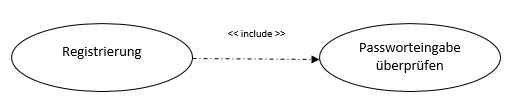
\includegraphics[scale=1]{Include_Use-Case.JPG}
\\
\footnotesize Abbildung 1: Include-Beziehung
\normalsize
\\
\\
\\
\textbf{Extend-Beziehung:}
\\
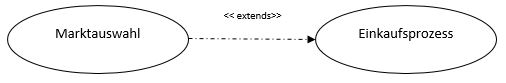
\includegraphics[scale=1]{Extend_Use-Case.JPG}
\\
\footnotesize Abbildung 2: Extend-Beziehung
\normalsize
\\
%\newpage
\subsection{Projektorganisation}
%MH: ich weis ja nicht wer von euch welchen teil geschrieben hat, aber ich würde mich inhaltlich gern nochmal über diese Absatz unterhalten
%AK: haben uns ja darüber bereits unterhalten- Änderung am 23.12. vorgenommen
Am 02. Oktober 2015 fand das erste Meeting mit der gesamten Projektgruppe der EinkaufsApp statt, hierbei wurden Absprachen über das weitere Vorgehen und die Projektumsetzung der Ideen und Ziele getroffen.
Das gesamte Team teilte sich zur optimalen Zielerfüllung in die Untergruppen Dokumentation, Design und Entwicklung auf.
Der Projektleiter und in diesem Falle auch Projektmanager wurde ebenso an diesem Tag ernannt.
Als Projektmanager war er nun für die Team- und Projektorganisation zuständig. Dazu gehört unter anderem das Einhalten der Projekt- und Meilensteinplanung und das Erfüllen der Projektziele.
Jegliche Unterhaltung basierte auf Mailverkehr oder fand durch Telefonkonferenzen statt. Jede Untergruppe musste sich selbst organisieren und wöchentlich ein Update dem Projektleiter zukommen lassen. Jeden Montag fanden Status-Telefonkonferenzen statt, wo sich alle Teammitglieder zusammenfanden und über den aktuellen Stand der Untergruppen informierten und über aufgekommene Probleme diskutierten. 
Die Untergruppen einigten sich außerdem auf Tools, die effizient und sinnvoll zur Umsetzung der anstehenden Aktivitäten und zum Einhalten der Projektziele verwendet wurden. 
%AK-Änderung-Ende

%\newpage
\subsubsection{Anforderungskatalog}
%MH: wenn die Doku parallel zur Implementation entstanden ist können hier nicht "ziele für das Projekt" definiert werden (das wäre wieder Planungsphase) --> %AK hab es nun geändert und den Satz raus genommen
In dem hier angeführten Kapitel werden konkrete Ziele für das bevorstehende Projekt formuliert, die auf den zuvor aufgeführten Funktionen der Applikation basieren.
Die einzeln genutzten Tools die im Pflichtenheft, welches sich im Anhang befindet, festgehalten sind, werden hier den einzelnen Arbeitsgruppen zugewiesen.
\\
%MH: in dem Bild sollte bei "Umgesetzt von" sollte eher stehen "Entwicklung" oder wahlweise von den "Entwicklern"
%MH: insgesammt bitte nochmal mit mir über die Organisation der Tabelle sprechen! und wenn möglich könnte es geminhin sinvoll sein PDFs einzubinden anstatt von bildern

%way to go for graphics
%negative \hspace um das bild nach links zu verschieben und trim um nicht die ganzen weißen bereiche der pdf zu übernehmen
\hspace*{-10mm} 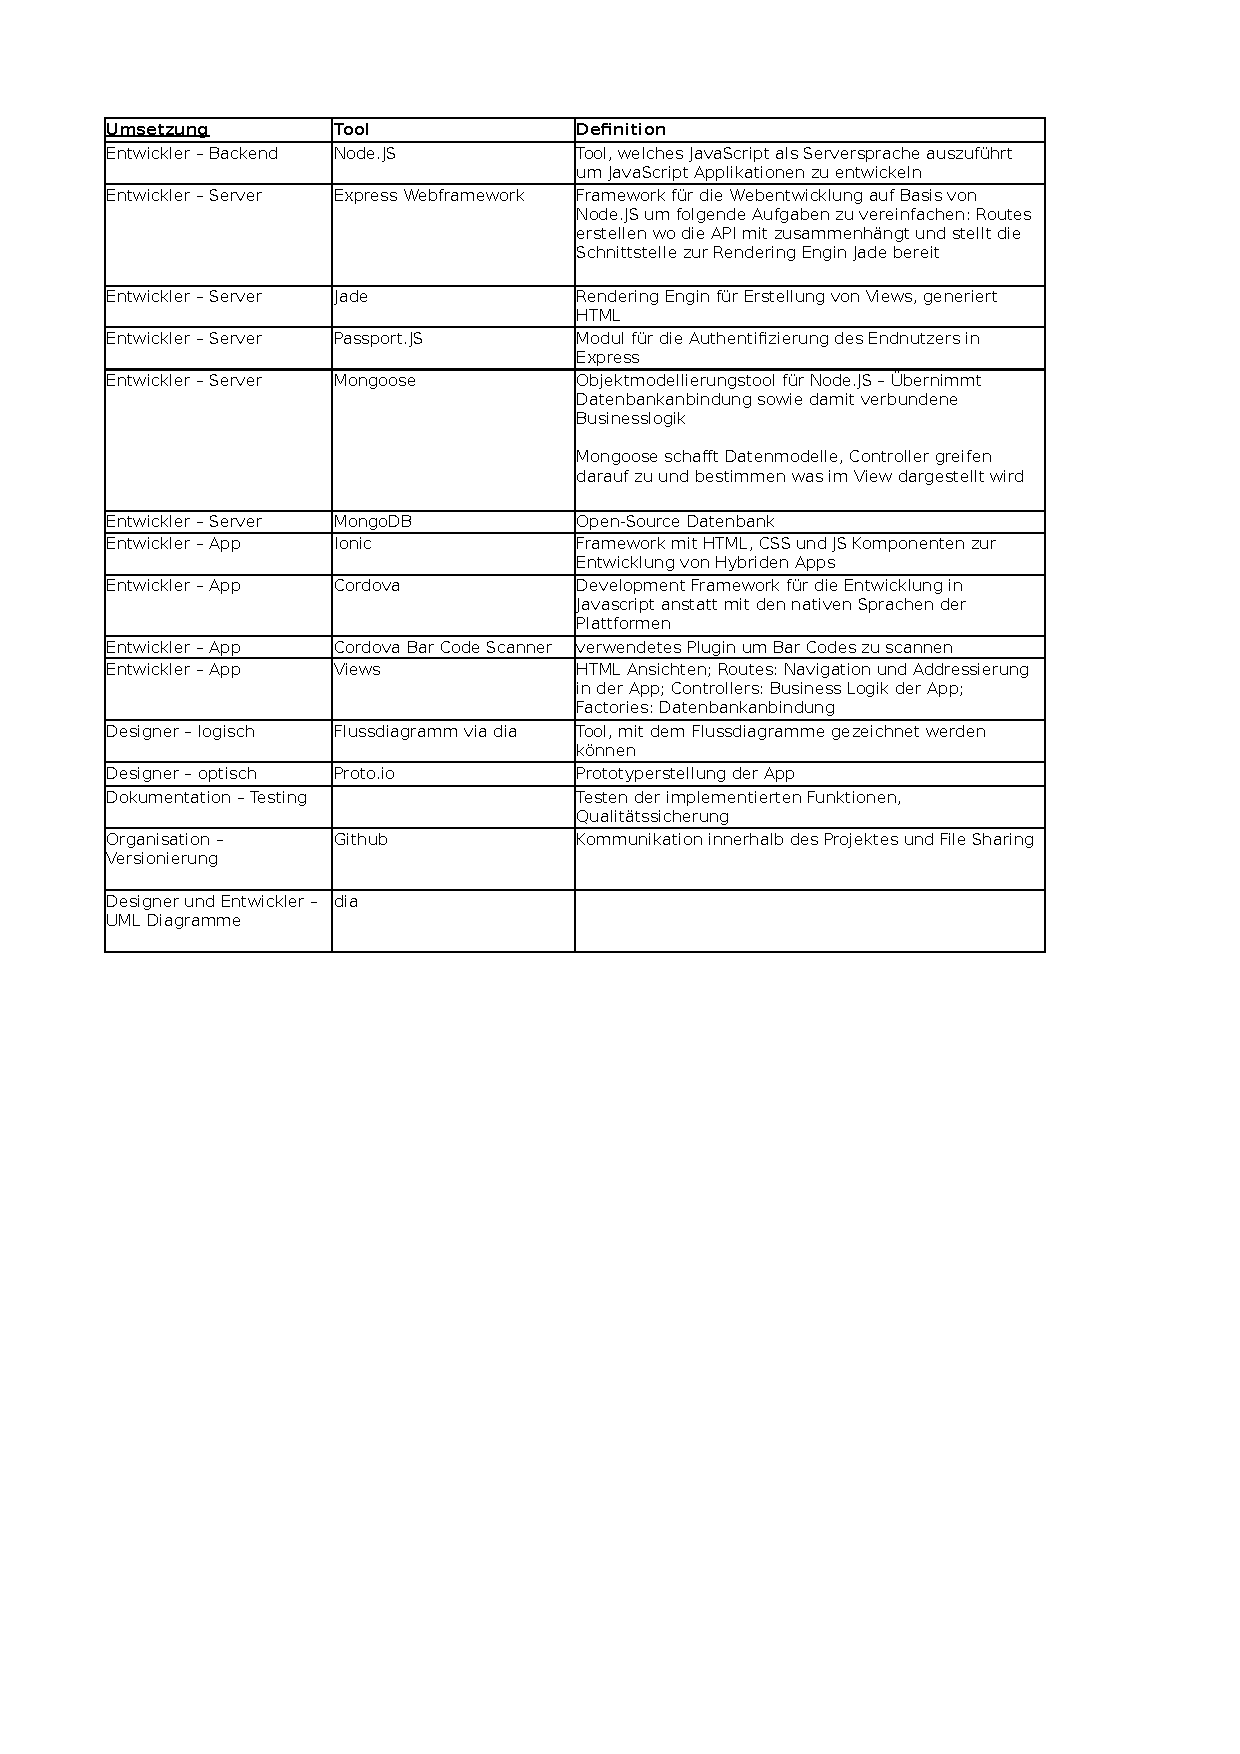
\includegraphics[trim = 17mm 130mm 0mm 20mm]{Anforderungskatalog.pdf}
\\
\\
\footnotesize Tabelle 1: Anforderungsanalyse
\normalsize
\\
\newpage
\subsubsection{Ist-Analyse}
Aus vorangegangener Erfahrung mit dem Thema der automatisierte Unterstützung durch eine App bei Einkäufen im privaten Bereich ist ein Grobkonzept, eines ER-Modells, bereits in das Projekt überführt worden. Dieses wurde verwendet, um ein Grundverständnis beim Designen und Implementieren zu erzeugen. 
\\
\\
\hspace*{-20mm} 
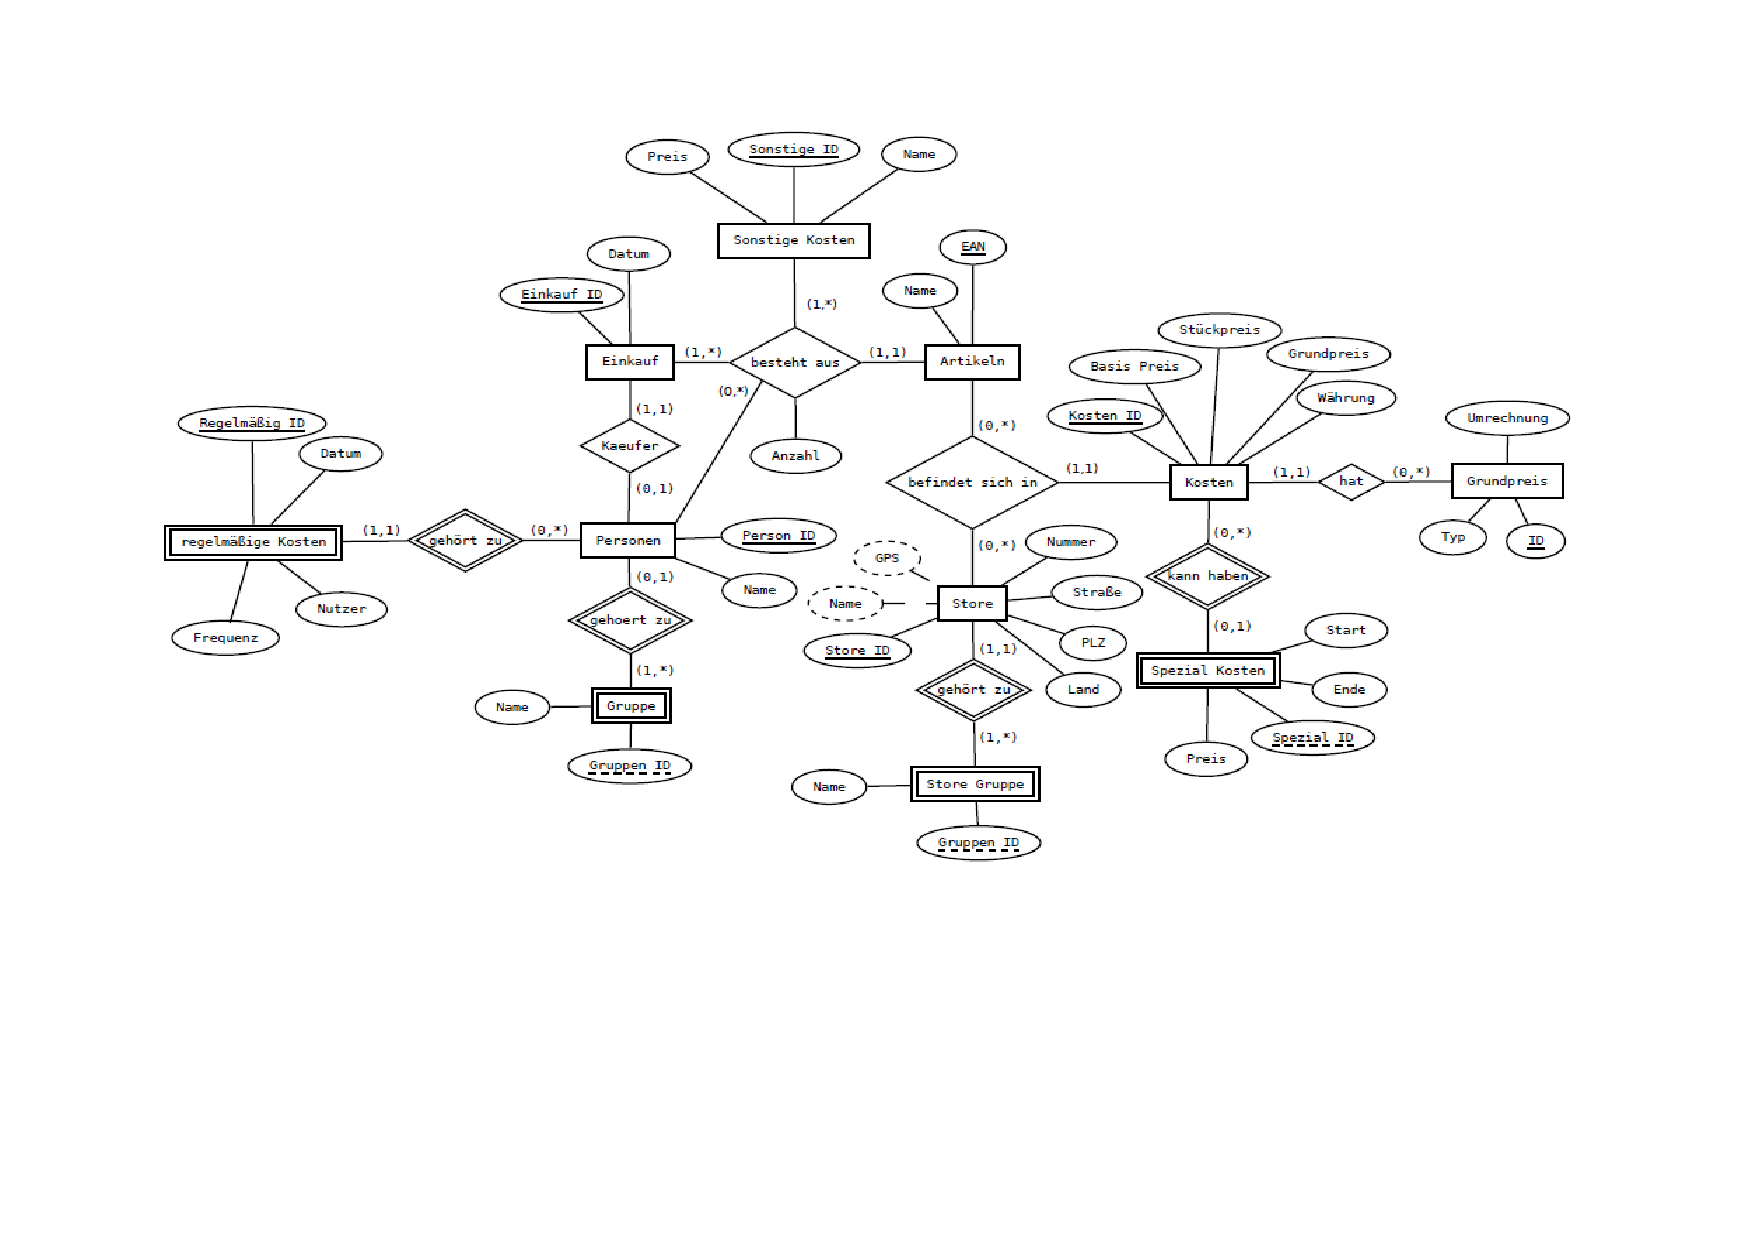
\includegraphics[trim = 15mm 40mm 0mm 20mm, clip, scale=0.7]{ER-Modell.pdf}
\linebreak
\footnotesize Abbildung 3: ER - Modell
\\
\normalsize
\linebreak
\\
Zu Beginn wurden die jeweiligen Kompetenzen der Projektmitarbeiter vor der Durchführung des Projektes aufgenommen. 
Aus diesen leiteten sich die Zugehörigkeiten jeder einzelnen Person in die Projektgruppen Dokumentation, Entwicklung und Design ab. 
\\
\\
\hspace*{-10mm} 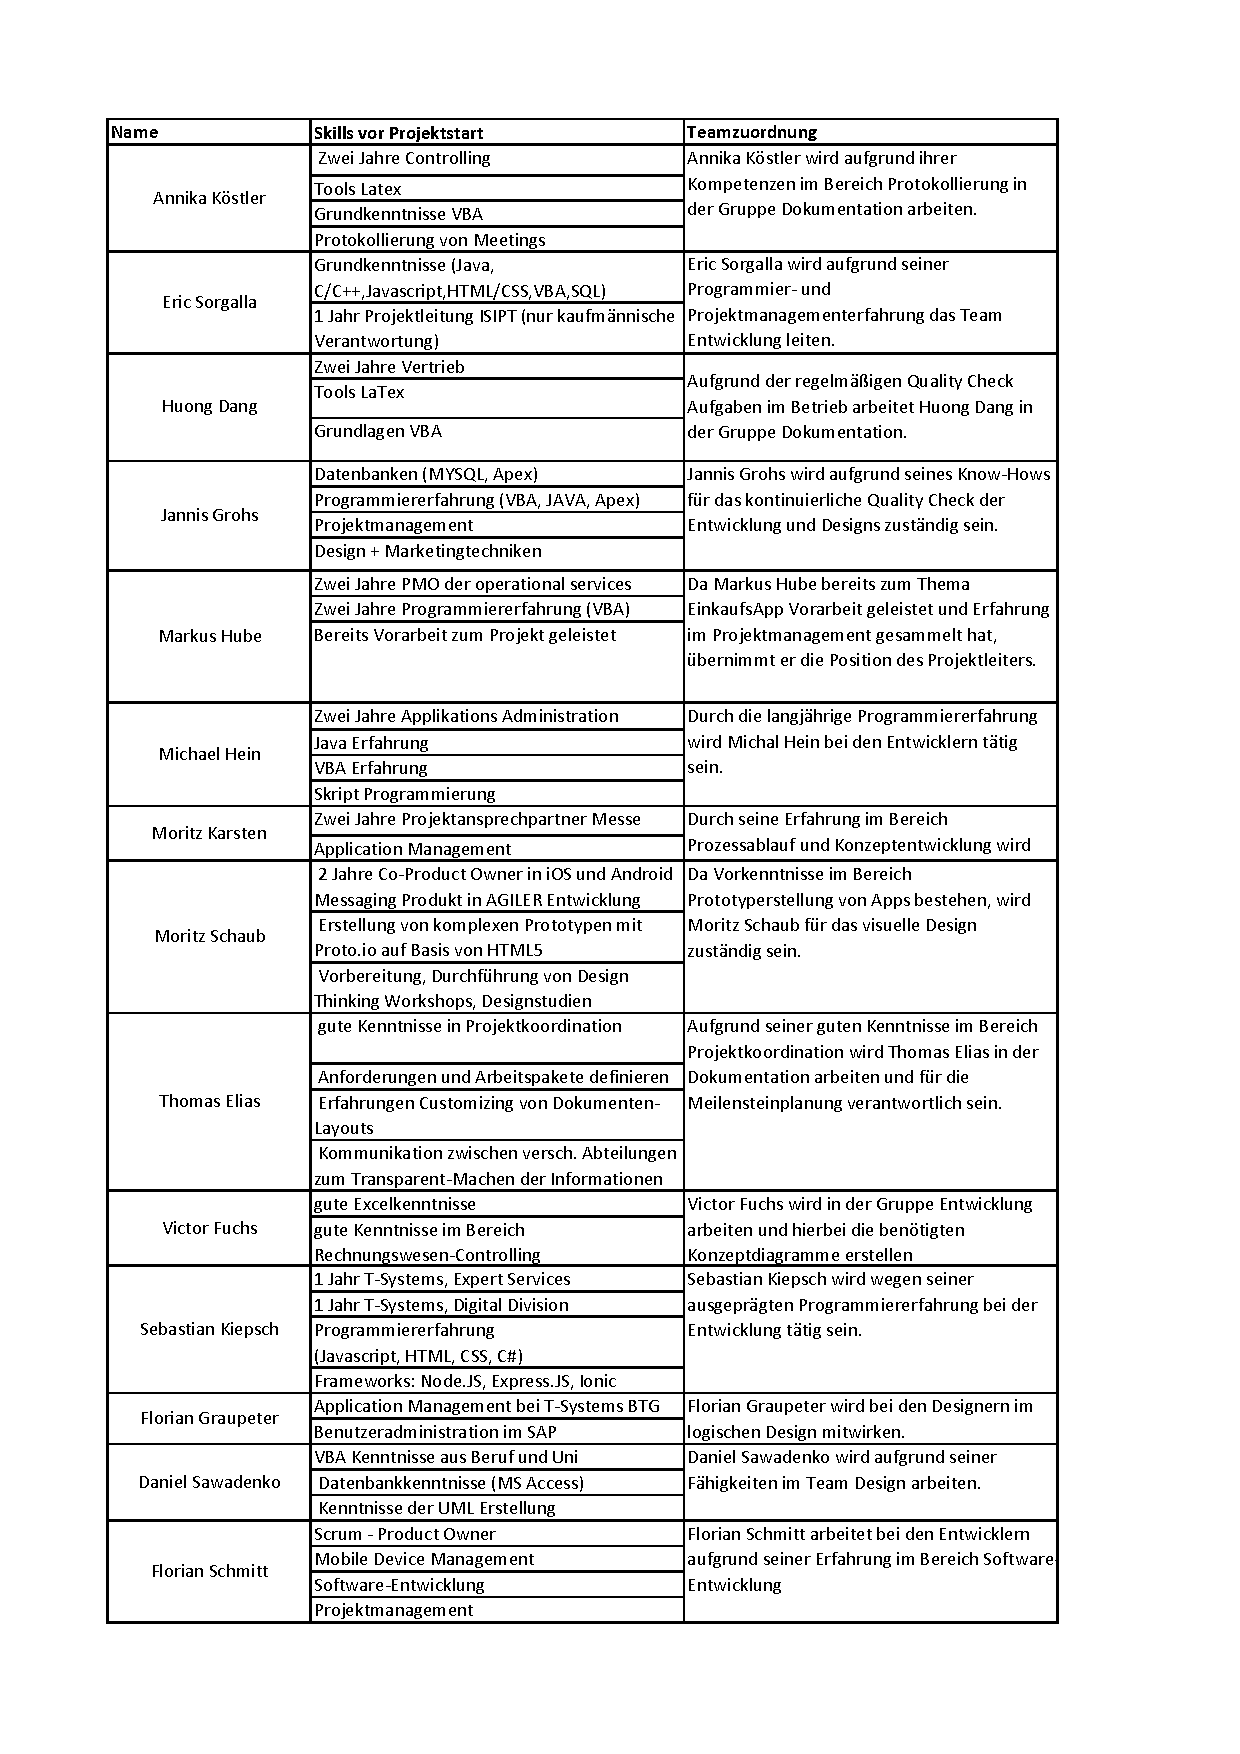
\includegraphics[trim = 15mm 0mm 0mm 20mm,clip,scale=0.8]{Skillliste.pdf}
\linebreak
\footnotesize Tabelle 2: Ist-Analyse
\\
\normalsize
\linebreak
\\
\newline
\newline
Insgesamt gibt es demnach drei Designer, fünf Entwickler und drei Dokumentatoren, die parallel den stetigen Quality Check durchführen.
\\
\subsubsection{Arbeitsplanung}
Zu Beginn der Projektorganisation wurde von der Dokumentation ein grober Plan erstellt, der eine Einteilung der Teams in organisatorische Einheiten aufzeigt und einen Rahmen für die Planung der Aufgaben, beziehungsweise Arbeitspakete, vorgibt. 
Es wurde ein organisatorisches Grundgerüst geschaffen, das allen Gruppen als Orientierung dient und gleichzeitig zur eigenständigen Organisation, sowie Bearbeitung der Arbeitspakete motiviert:
\\
\\
%MH: hier taucht wieder die Planungsphase auf...
\hspace*{-10mm} 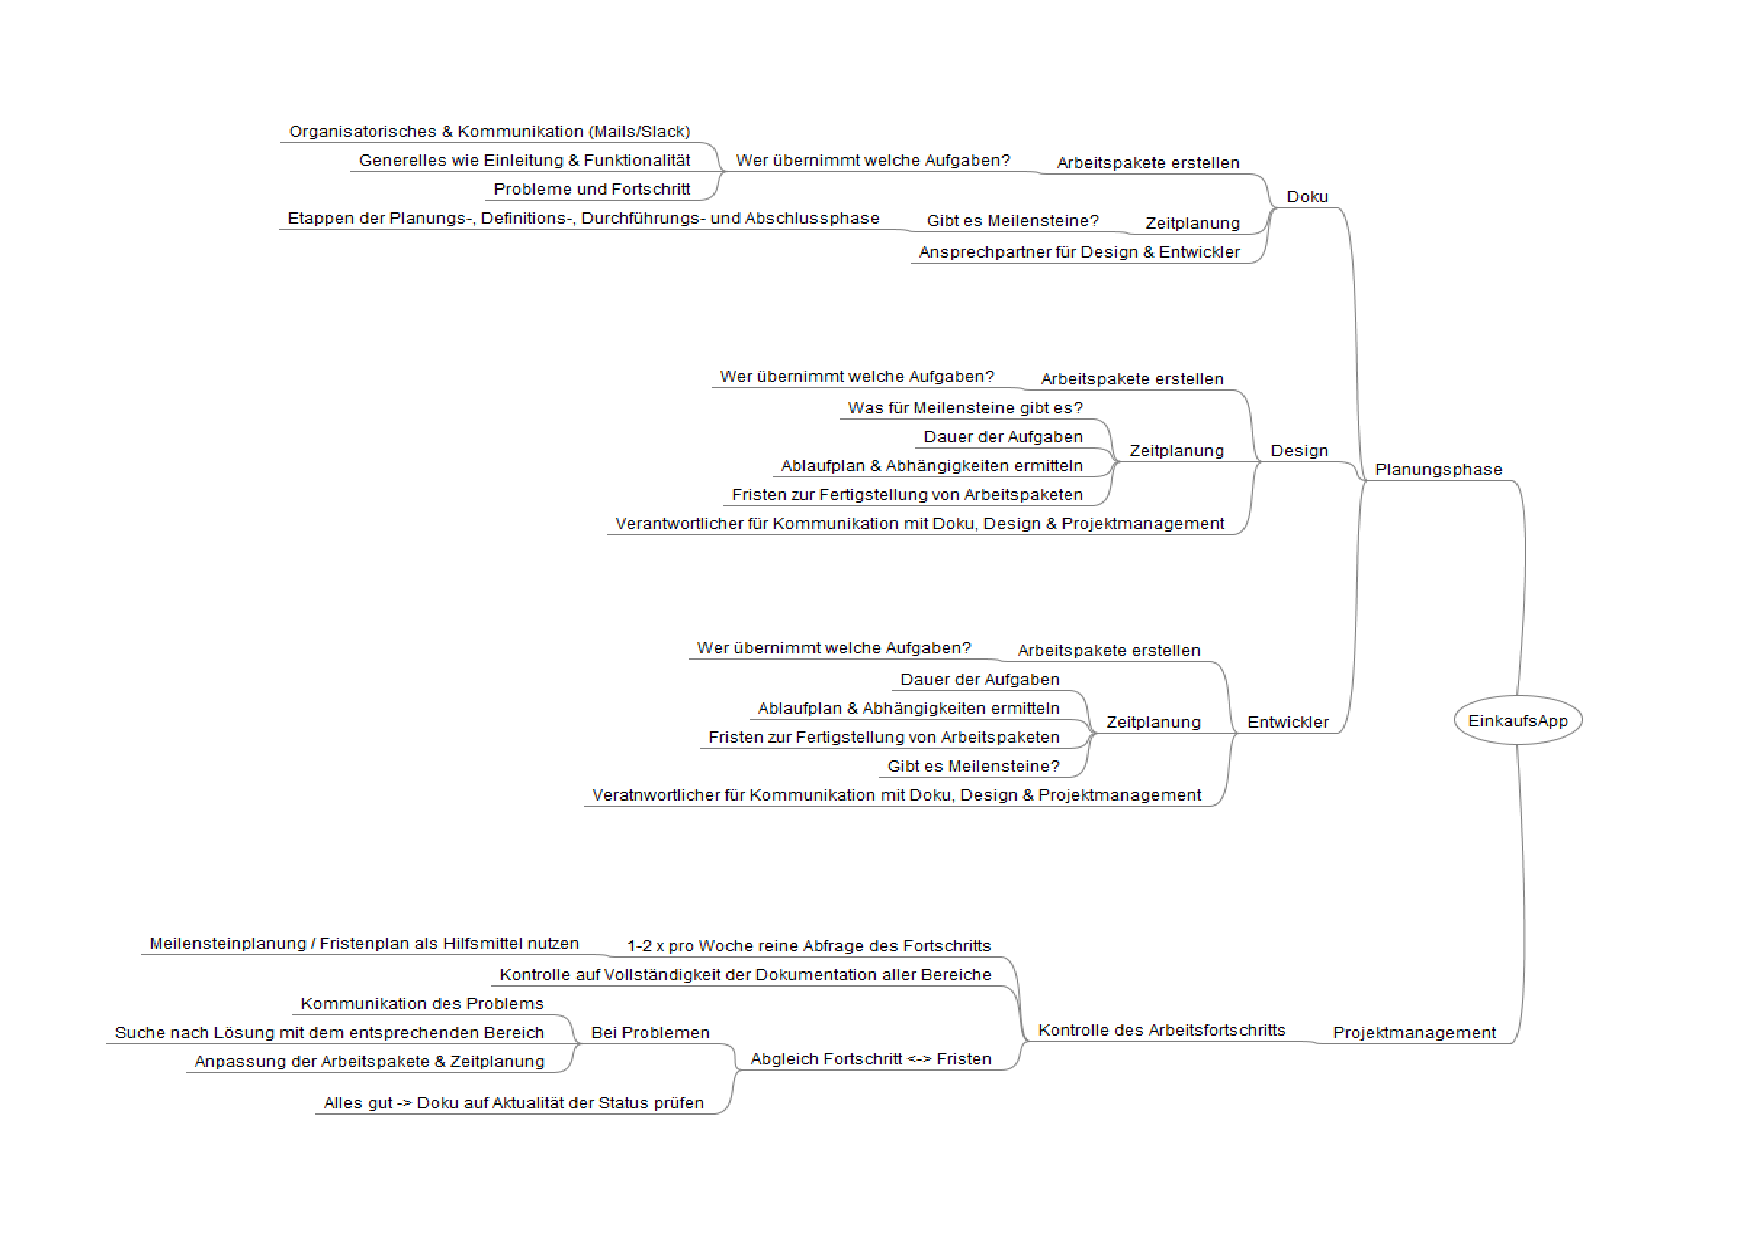
\includegraphics[trim = 20mm 0mm 0mm 20mm,clip,scale=0.7]{Aktivitaetsliste.pdf}
\\
\footnotesize Abbildung 4: Aktivitätsliste
\normalsize
\\
\linebreak
\subsubsection*{Meilensteinplanung}
Mithilfe der erstellten Meilensteinplanung wurde das pünktliche Erreichen der Projektziele geplant.
Jedes Team konnte sich an dieser Tabelle orientieren und seine Aufgaben der Reihe nach ordnen und ausführen.
\\
\\
\hspace*{-10mm} 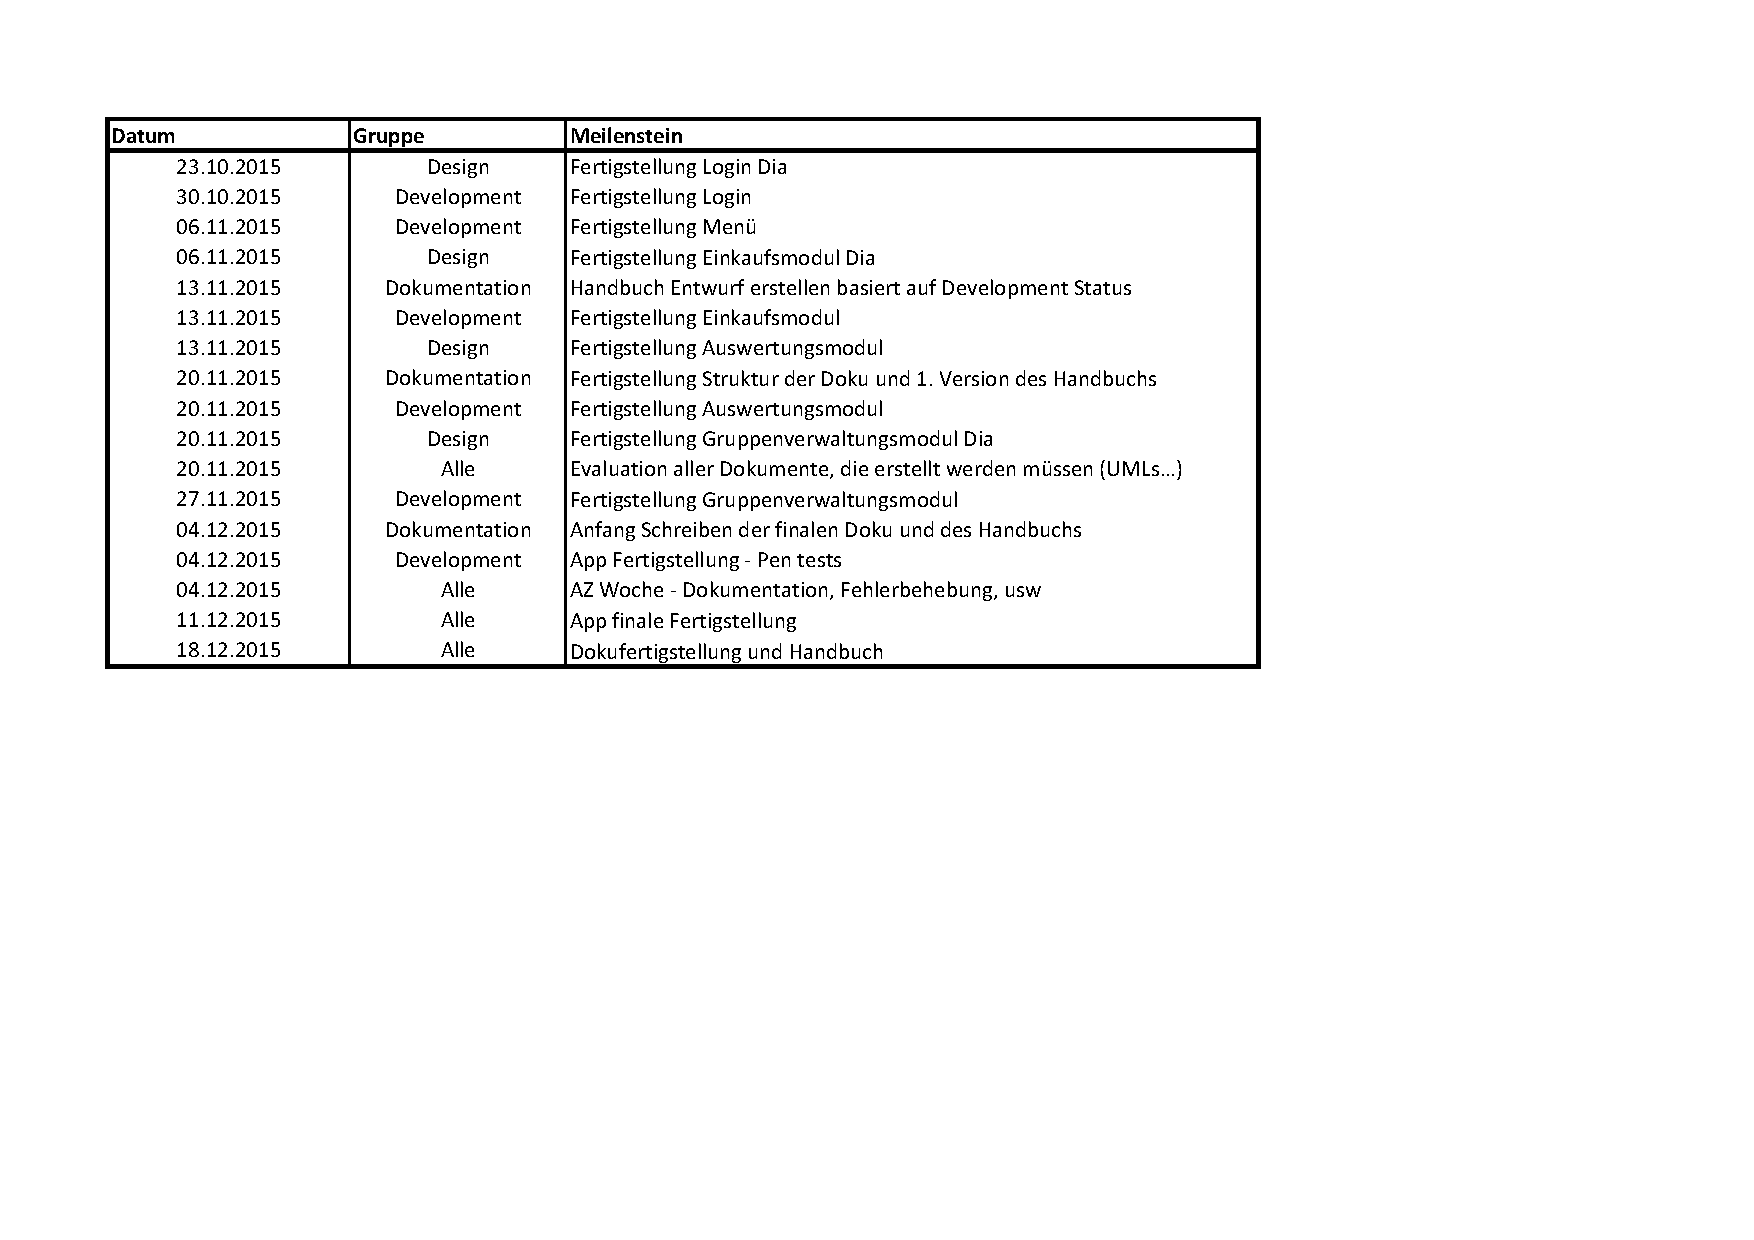
\includegraphics[trim = 10mm 90mm 10mm 20mm,clip, scale=0.9]{Meilensteine.pdf}
\\
%MH: holt euch ganz schnell nochmal fixierte Aussagen dazu von Eric, wenn er euch dazu überhaupt etwas sagen kann. Wenn nicht komplett anders darstellen oder rausnehmen.
\footnotesize Tabelle 3: Meilensteine
\normalsize

\subsubsection{Agiles Projektmanagement}
Nachdem ein grober organisatorischer Rahmen für das Projekt von der Gruppe Dokumentation vorgegeben wurde, haben die einzelnen Gruppen, durch agile Projektmanagement-Methoden,  ihre Arbeitspakete und Ablaufpläne festgelegt. 
Die Dokumentation erstellte Arbeitspakete für alle Gruppen und jedes Projektmitglied hat sich nach dem Pull-Prinzip – bekannt aus der Projektmanagement-Methode Kanban – seine Arbeitspakete abgeholt und eine Bearbeitungsfrist definiert. 
In der Gruppe der Entwickler wurde unter Zuhilfenahme des Tools „Trello“ die Planung und Durchführung der Arbeitspakete definiert. Trello ist ein Web-Dienst, der ein Board anbietet, um Arbeitspakete gemäß agiler Projektmanagement-Methoden zu bearbeiten und Arbeitsfortschritte transparent darzustellen. 
Die Designer haben ihre Arbeitspakete auf Basis eines Ablaufplanes verteilt. Es wurden die Phasen Prototyp-Entwurf, Prototyp-Review, Prototyp-Modifikationen und Prototyp-Test und Prototyp-Abnahme durchlaufen.
\newpage
\subsection{Sicherheit}
%AK-28.12.5-Bearbeitung Anfang
Sobald Daten eines Nutzers für eine Applikation gespeichert werden, wird ein gewisser Standard an Sicherheit gefordert, damit keinen Dritten diese Daten zugänglich werden.
In der EinkaufsApp wurden folgende Maßnahmen getroffen um dies gewährleisten zu können:
\\
Einige konkrete Sicherheitsvorkehrungen lauten:
\\
1)	Eine Session läuft nach 10 Minuten ohne Request an den Server ab.
\\
2)	Jedes Passwort wird als Einweg-Hash in der DB gespeichert.
\\
3)	Es wird eine Authentifizierung durchgeführt, das heißt ein Sicherstellen, dass die beteiligten Parteien auch tatsächlich die sind, die sie vorgeben zu sein.
\\
4)	Data Security: Eine weitere wichtige Technik zur Sicherheit von Webanwendungen spielt das SSL-Protokoll (Secure Socket Layer). Bei Verwendung dieser Protokolle wird vor der eigentlichen HTTP-Kommunikation ein geschützter Kanal aufgebaut, 
sodass die Nutzerdaten für Dritte nicht zugänglich sind. Die Nutzerdaten werden in einem normalen Web-Formular eingetragen (Login-Screen) und mittels POST-Request an den Server gesendet. Da der TCP-Kanal abgesichert ist, haben Dritte keinen Zugriff auf die 
Nutzdaten innerhalb des POST-Requests, d.h. Nutzername und Passwort werden gesichert übertragen.
%AK-28.12.15-BearbeitungEnde
%\newpage
\section{Durchführungsphase}

In diesem Abschnitt wird die Funktionsweise der EinkaufsApp beschrieben. Dabei werden die einzelnen Hauptprozesse separat vorgestellt und deren technische Umsetzung erläutert. Die Hauptprozesse sind unterteilt in den Login und die Registrierung des Nutzers, den Einkaufsprozess, die Nutzerverwaltung und die Auswertung. 
Generell wurde in der Entwicklung nach dem Modell-View-Controller Prinzip gearbeitet. Nachdem die Prozesslogik der Designer stand („Modell“), wurden die einzelnen Views, also die visuelle Darstellung, der zu implementierten Funktion, die der Nutzer am Ende sieht, entwickelt und welche schlussendlich über die „Controller“ mit der Logik versehen wurden. Jedes einzelne View hat dabei seine eigene Route.

\subsection*{Einleitung}
Die genannten Hauptprozesse stehen, wie in dem folgenden Diagramm zu sehen ist, in Relation. Dabei wurden die Views\footnote {In der EinkaufsApp werden Views verwendet, da die Systemarchitektur auf der Model-View-Controller Architektur basiert.}  als einzelne Klassen dargestellt:
\\
\\
%MH: ist dem Leser an der stelle Klar was "Views" sind???
%AK: jetzt ja :)
\hspace*{-10mm} 
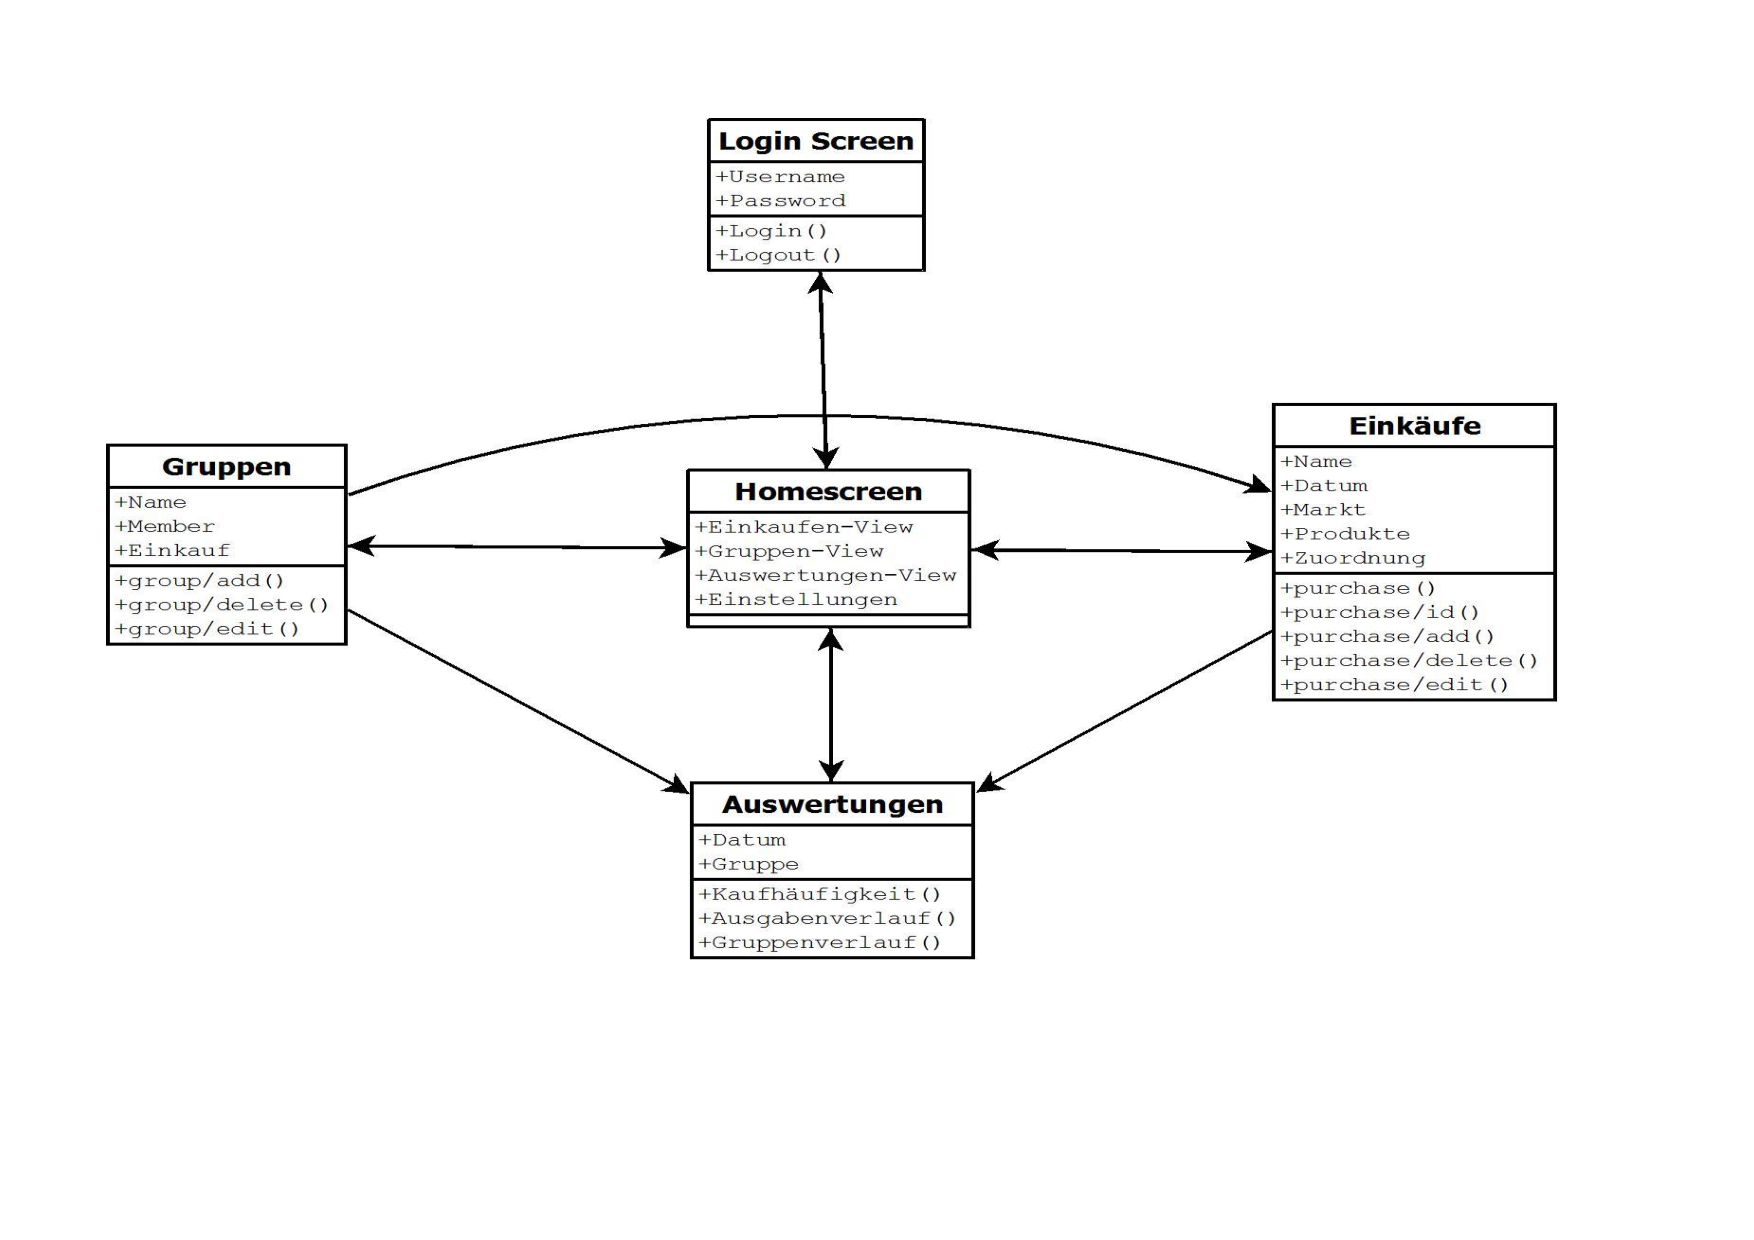
\includegraphics[trim = 17mm 30mm 0mm 20mm,clip,scale=0.7]{Klassendiagramm.pdf}
\\
\footnotesize Abbildung 5: Klassendiagramm
\normalsize

\subsection{Architektur}

Die App selbst wurde auf Basis des Ionic Frameworks Entwickelt, der Webserver wurde mittels Node.JS umgesetzt und die zugrundeliegende Datenbank ist eine MongoDB. Die Entscheidung zu diesen Komponenten fand auf Grund ihres guten Zusammenspiels hinsichtlich Webapplikationen statt. Im ersten Schritt wurde die MongoDB gewählt, weil es für unsere Zwecke eine angemessene Flexibilität aufgrund der Schemalosigkeit bietet, aber auch die Skalierbarkeit einer NoSQL für den Aspekt der Zukunftssicherheit mit sich bringt. Node.JS ist besonders gut geeignet, um weniger rechenintensive Aufgaben, wie das Handeln einer Anfrage und das Verweisen auf eine Ressource, auf einem Server umzusetzen. Ebenfalls wurde diese Entscheidung durch das gute Zusammenspiel mit MongoDB und Mongoose bestärkt. 
\\
Das Ionic Framework wurde allem voran genutzt, weil ermöglicht, ein zeitgemäßes Desing zu erstellen und die Möglichkeit bietet, sowohl Android, als auch iOS-lauffähige Anwendungen zu erstellen, ohne dafür zusätzliche Entwicklungsarbeit zu leisten.
Für detailliertere Ausführungen wird auf das Pflichtenheft verwiesen.

\subsection{Registrierung}
Um die EinkaufsApp zu nutzen, muss sich jeder Nutzer mittels einer E-Mail-Adresse und einem Kennwort für der App registrieren.
Eine Registrierung ist bei dieser App unentbehrlich, da für jeden Nutzer ein Profil angelegt wird und diesem Profil innerhalb der Datenbank die Produkte und Finanzen zugeordnet werden.
In den folgenden Unterpunkten wird der Prozess der Registrierung jeweils von den Designern und Entwicklern beschrieben.
\subsubsection*{Design}
Die Designer haben zu der Registrierung und zu dem Login, welcher im Punkt 3.4 behandelt wird, das folgende Flussdiagramm entworfen:
\\
\hspace*{-10mm} 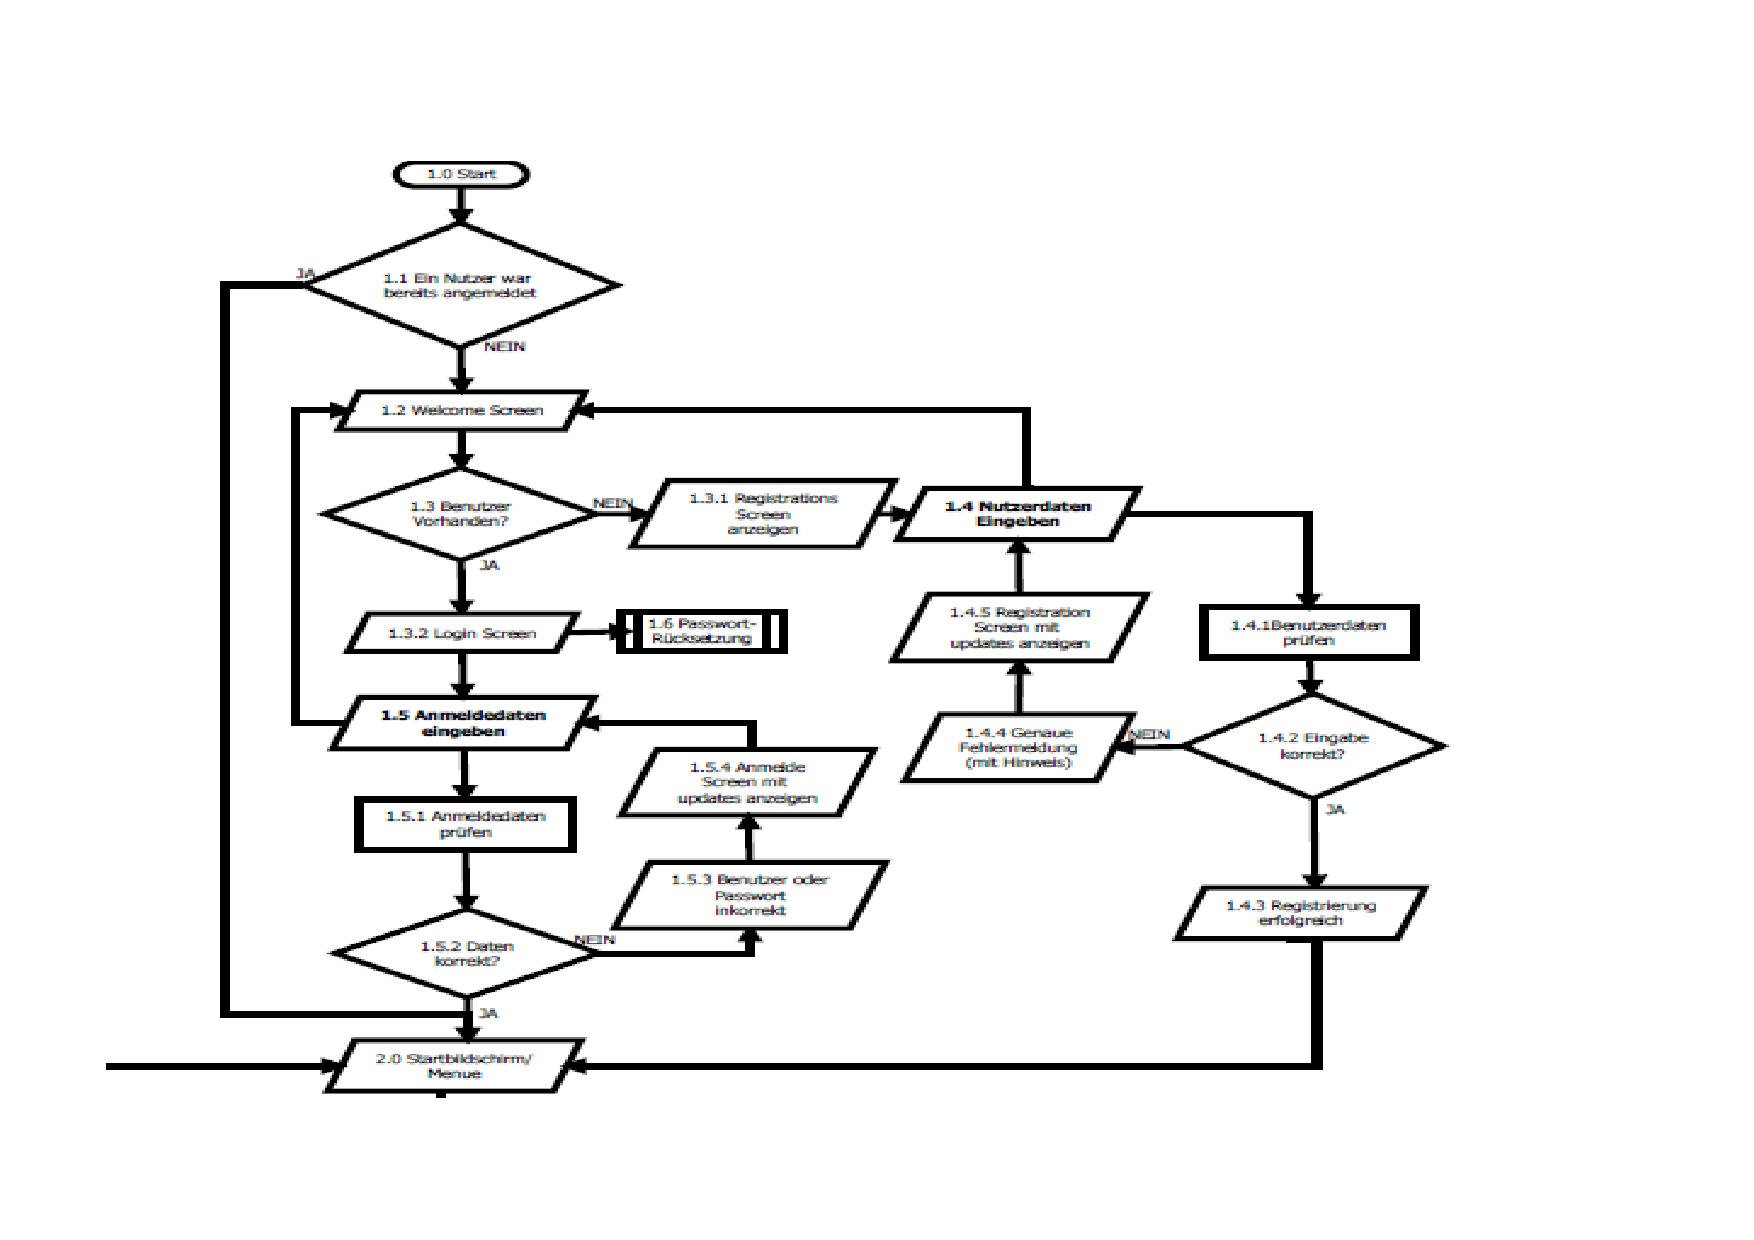
\includegraphics[trim = 17mm 0mm 0mm 20mm, clip, scale=0.8]{Login-PDF.pdf}
\footnotesize Abbildung 6: Flussdiagramm Login
\normalsize
\\
\linebreak
Das Flussdiagramm beschreibt sukzessiv den Ablauf des Registrierungs- und des Loginvorgangs, welcher von den Entwicklern daraufhin technisch umgesetzt wurde.
%\newpage
\subsubsection*{Entwicklung}
Die Entwickler befassten sich mit den Funktionen der Applikation und sorgten bei der Registrierung dafür, dass alle Daten ordnungsgemäß geprüft und in die Datenbank eingepflegt werden.
%Als Datenbank wird für die App MongoDB genutzt, welche via RoboMongo gemanagt wird. Als Programmiersprache kommt JavaScript zum Einsatz.
%HD 01.01.15: Stimmt das so? ich denke jetzt eher im Angebot. Ich änder das mal!
%MH 01.01.16: ich hab mal den zweiten satz auskommentiert. der ist inhaltlich schon richtig, sollte nur an anderer stelle auftauchen (ich hatte da irgendwo doch mal einen absatz zur architektur geschrieben), bleibt die frage ob der eine satz alles ist was man hier zur entwicklung sagen kann (passwortsicherheit und so?) - und huong... seit heute haben wir 2016^^
\footnote{Genaueres zu der Datenstruktur können Sie dem angehängten Angebotsdokument entnehmen.} verwendet.

Bei der Registrierung werden die einzelnen Benutzereingaben durch bestimmte Regeln in Hinblick auf Länge, E-Mail-Format, Eindeutigkeit, sowie Sicherheitskriterien bei der Passwortvergabe in der Applikation geprüft.\footnote{Die konkreten Regeln der Benutzereingaben können Sie in dem angehängten Handbuch entnehmen.}

Wenn alle Prüfungen erfolgreich waren, wird der Benutzer angelegt und das Passwort verschlüsselt in Form eines Hashs in der Datenbank gespeichert.
%\newpage
\subsection{Login}
\subsubsection*{Design}
Das Flussdiagramm der Designer für den Login ist im Abschnitt 3.3 Registrierung zu finden. 
\subsubsection*{Entwicklung}
Die Entwicklung beschäftigt sich mit der Funktionsweise des Logins und prüft hierbei, ob der Benutzer in der Datenbank existiert. Falls dies der Fall ist, wird das Passwort geprüft und bei korrekter Eingabe ist der Login erfolgreich durchgeführt.
Wenn der Benutzer sein Passwort vergessen hat, kann er dieses zurücksetzen lassen. Hierbei bekommt er eine E-Mail an die im Userprofil hinterlegte E-Mail Adresse. Diese Funktionalität ist bereits implementiert, wird aber auf Grund der Sicherheitsbestimmungen der Testumgebung geblockt. Diese enthält ein Token womit es einen Benutzer ermöglicht wird sein Passwort zu ändern. Dieses Token ist genau eine Stunde gültig, danach verfällt es. 
In dem dann aufgerufenen Bildschirm muss der Nutzer nun sein Passwort zweimal eintragen. Daraufhin ändert die Datenbank das Kennwort des Nutzer und speichert dieses.
%\newpage
\subsection{Marktauswahl}
Bevor der Einkaufsprozess beginnt muss der Nutzer einen Markt auswählen, hierfür wird der Standort des Nutzers ermittelt via GPS ermittelt und bereits registrierte Märkte in seiner Nähe angezeigt. 
\subsubsection*{Design}
Die Designer haben hierzu, ebenso wie bei der Registrierung und dem Login ein Flussdiagramm erstellt: 
\\
\\
\hspace*{-10mm} 
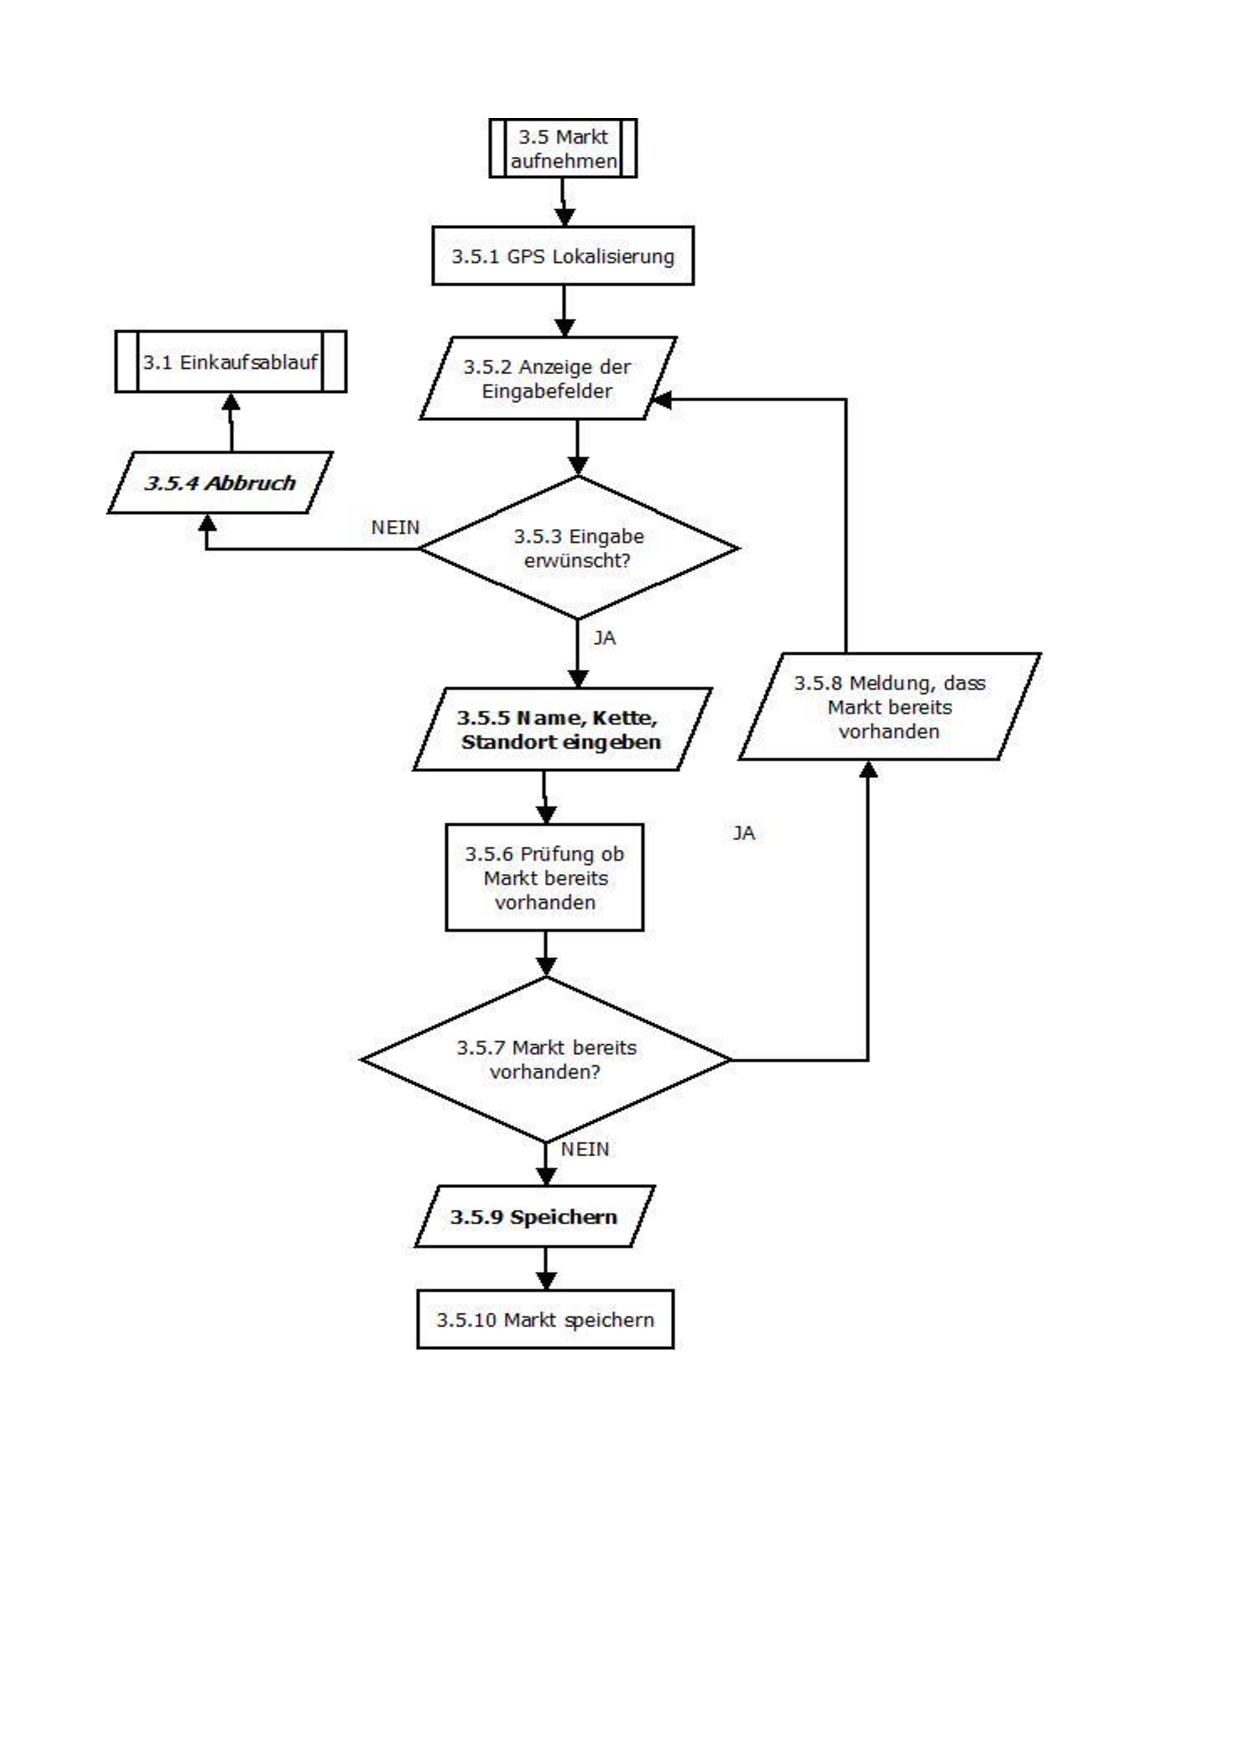
\includegraphics[trim = 17mm 40mm 0mm 20mm, clip, scale=0.8]{Markt-Aufnahme.pdf}
\\
\footnotesize Abbildung 7: Markt-Auswahl
\normalsize
\subsubsection*{Entwicklung}
Der vom Design erstellte Ablauf der Marktauswahl wird direkt in den Einkaufsprozess mit eingebunden. Sobald der Nutzer die Option „Einkaufen“ wählt gelangt dieser in den Marktauswahl-View.Anders als im geplanten Ablauf der Designer, kann der Nutzer selber entscheiden, in welchem Markt er sich gerade befindet, indem er entweder in der direkt aufgeführten Marktliste einen auswählt, oder die Option „Markt hinzufügen“ nutzt. Dies hat technische Gründe, da zurzeit eine Lokalisierung der Märkte via GPS aus Zeitgründen noch nicht umgesetzt wurde.
%HD - 23.12.2015 Ende
%\newpage
\subsection{Einkaufsverwaltung}
\subsubsection*{Design}
Aktivitätsdiagramm „Einkauf einlesen“ 
\\
\\
\hspace*{-10mm} 
%HD 01.01.16: Ich hab hier mal das DIagramm von Thomas eingepflegt, es sei denn wir müssen das Aktivitätsdiagramm drin lassen. Sagt bescheid
%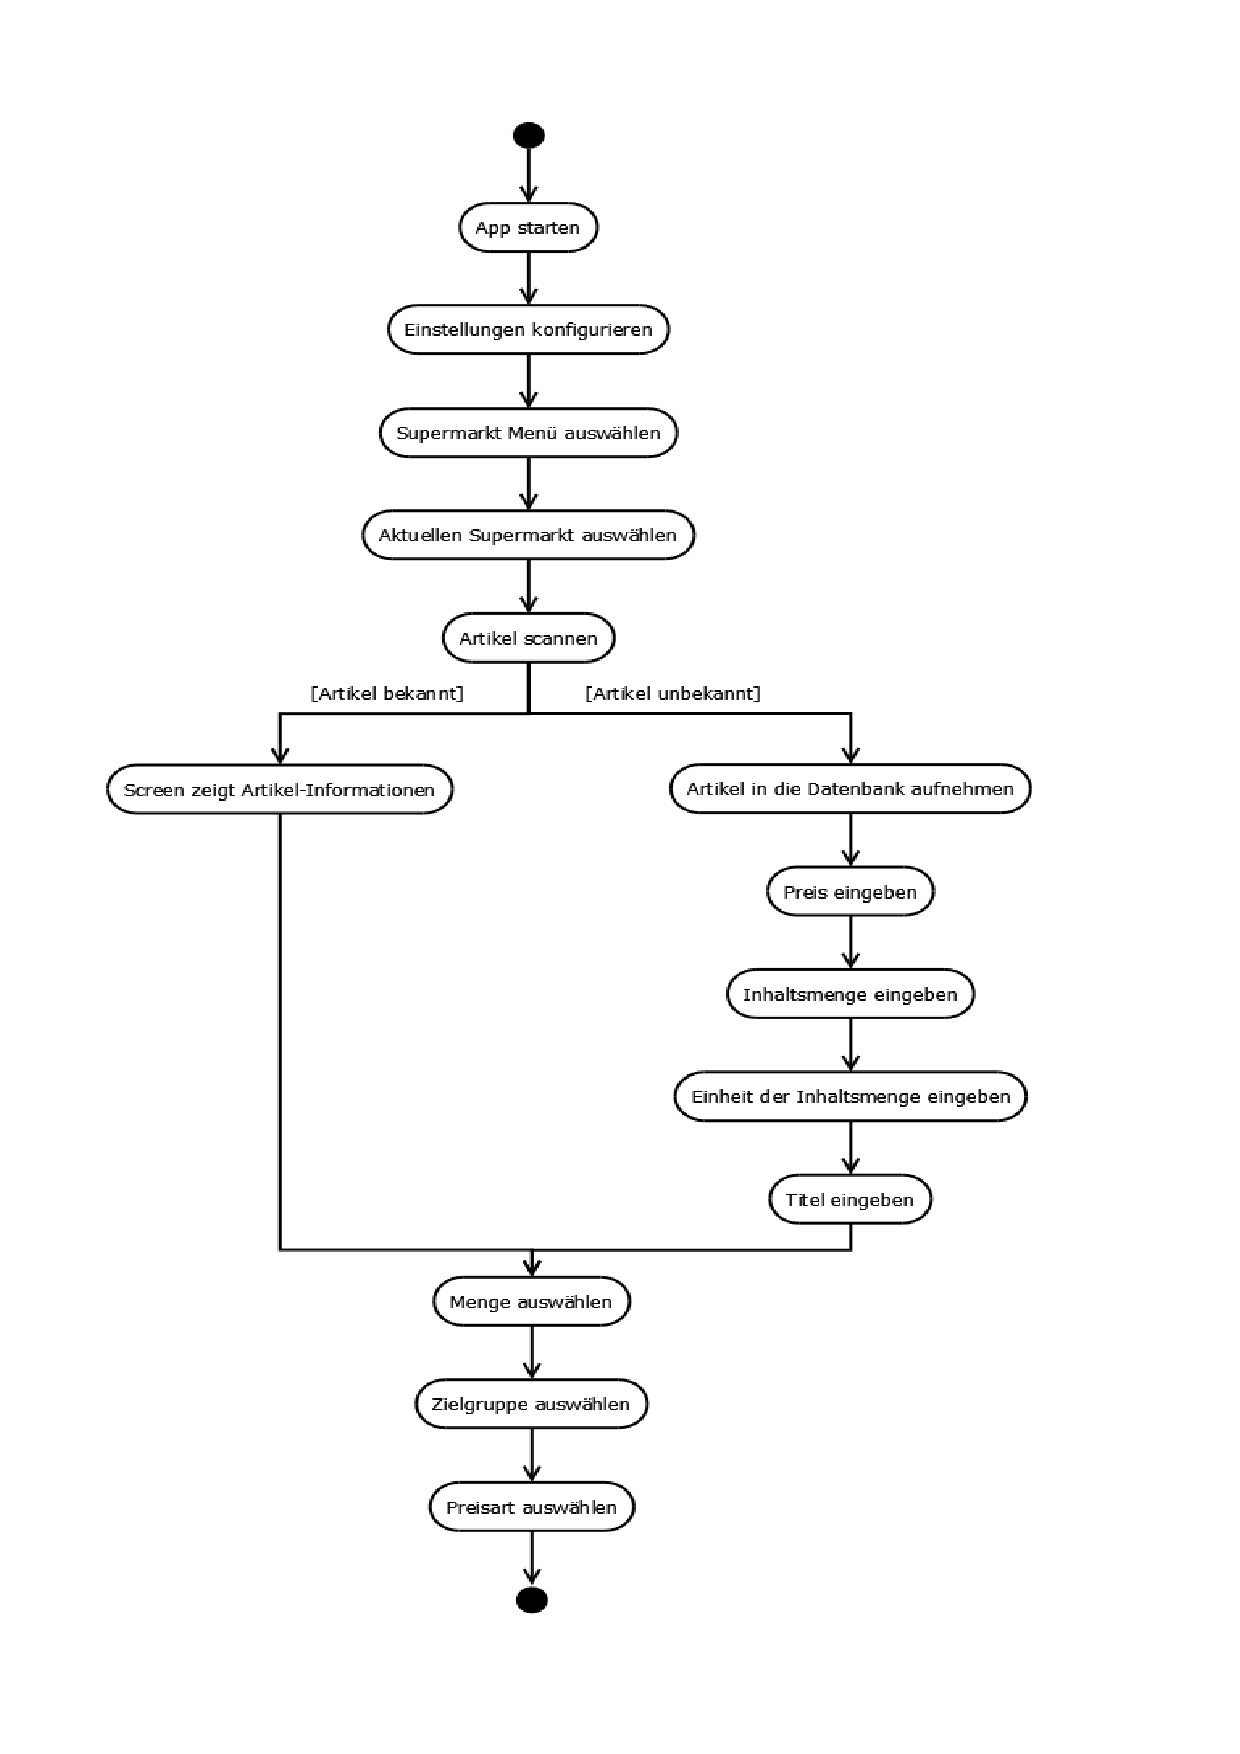
\includegraphics[trim = 17mm 0mm 0mm 20mm,clip, scale=0.7]{Aktiv-Einkauf.pdf}
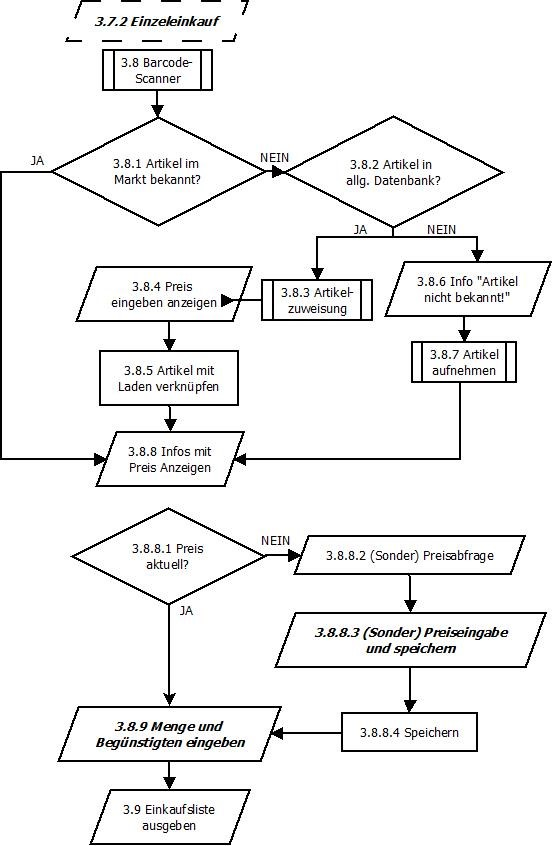
\includegraphics[scale=0.7]{Einzeleinkauf_Diagramm.jpg}
\\
\footnotesize Abbildung 8: Flussdiagramm-Einzeleinkauf
\\
\\
\normalsize
Das Design Team hat ein Flussdiagramm zur Einkaufsverwaltung erstellt, das den Ausbau der Systemarchitektur berücksichtigt und als Orientierung für die Entwickler gilt. Zwecks Übersichtlichkeit ist nur ein Teil des Flussdiagramms enthalten\footnote {Anm. d. Autors: Das vollständige Flussdiagramm befindet sich im Anhang}. 
\\
Gleichzeitig wird ein Prototyp in Proto.io entwickelt, mit der Zielsetzung, die Hauptfunktionalität der Anwendung abzubilden. Das Tool gibt bereits im frühen Projektstadium, vor der eigentlichen Entwicklung, ein Gefühl für das Endprodukt.
\\
Insbesondere bei der Umsetzung der Designvorgaben durch die Entwicklung ist es eine große Herausforderung sich untereinander abzustimmen und speziell die Umsetzbarkeit von Designvorgaben zu prüfen. 

\subsubsection*{Entwicklung}
Da das Projekt enorm zeitkritisch war sind Design und Implementation stark parallelisiert abgelaufen. Um innerhalb von zwei Monaten ein lauffähiges und qualitätsgesichertes Software Produkt zu erstellen bedarf es eines überschaubaren und für alle Mitglieder transparenten Projektes.
\\
Im Verlauf des Projektes wurde eine zusätzliche Organisationseinheit zwischen dem Gesamtprojekt und den einzelnen Entwicklern eingefügt, um einen besseren Überblick zu gewährleisten und schneller Entscheidungen treffen zu können. 
\\
Durch eine klare Aufgabentrennung, die anhand der einzelnen Module der EinkaufsApp abgegrenzt wurde, wurden die verschiedenen Kenntnisse der Entwickler berücksichtigt. 
\\
Zum Schluss mussten schließlich die Schnittstellen angepasst und die Kompatibilität der einzelnen Module geprüft werden

%TO DO - TE: einpflegen
%\newpage
\subsection{Nutzerverwaltung}
Die Nutzerverwaltung ermöglicht dem Nutzer die individuelle Zuweisung von anderen Accounts als Gruppenmitglieder zu bereits erstellten Gruppe. Ziel dessen ist die vereinfachte Finanzverwaltung wärend des Einkaufes, sowie die Möglichkeit komplexere Auswertung durchzuführen.

\subsubsection*{Design}
\hspace*{-10mm} 
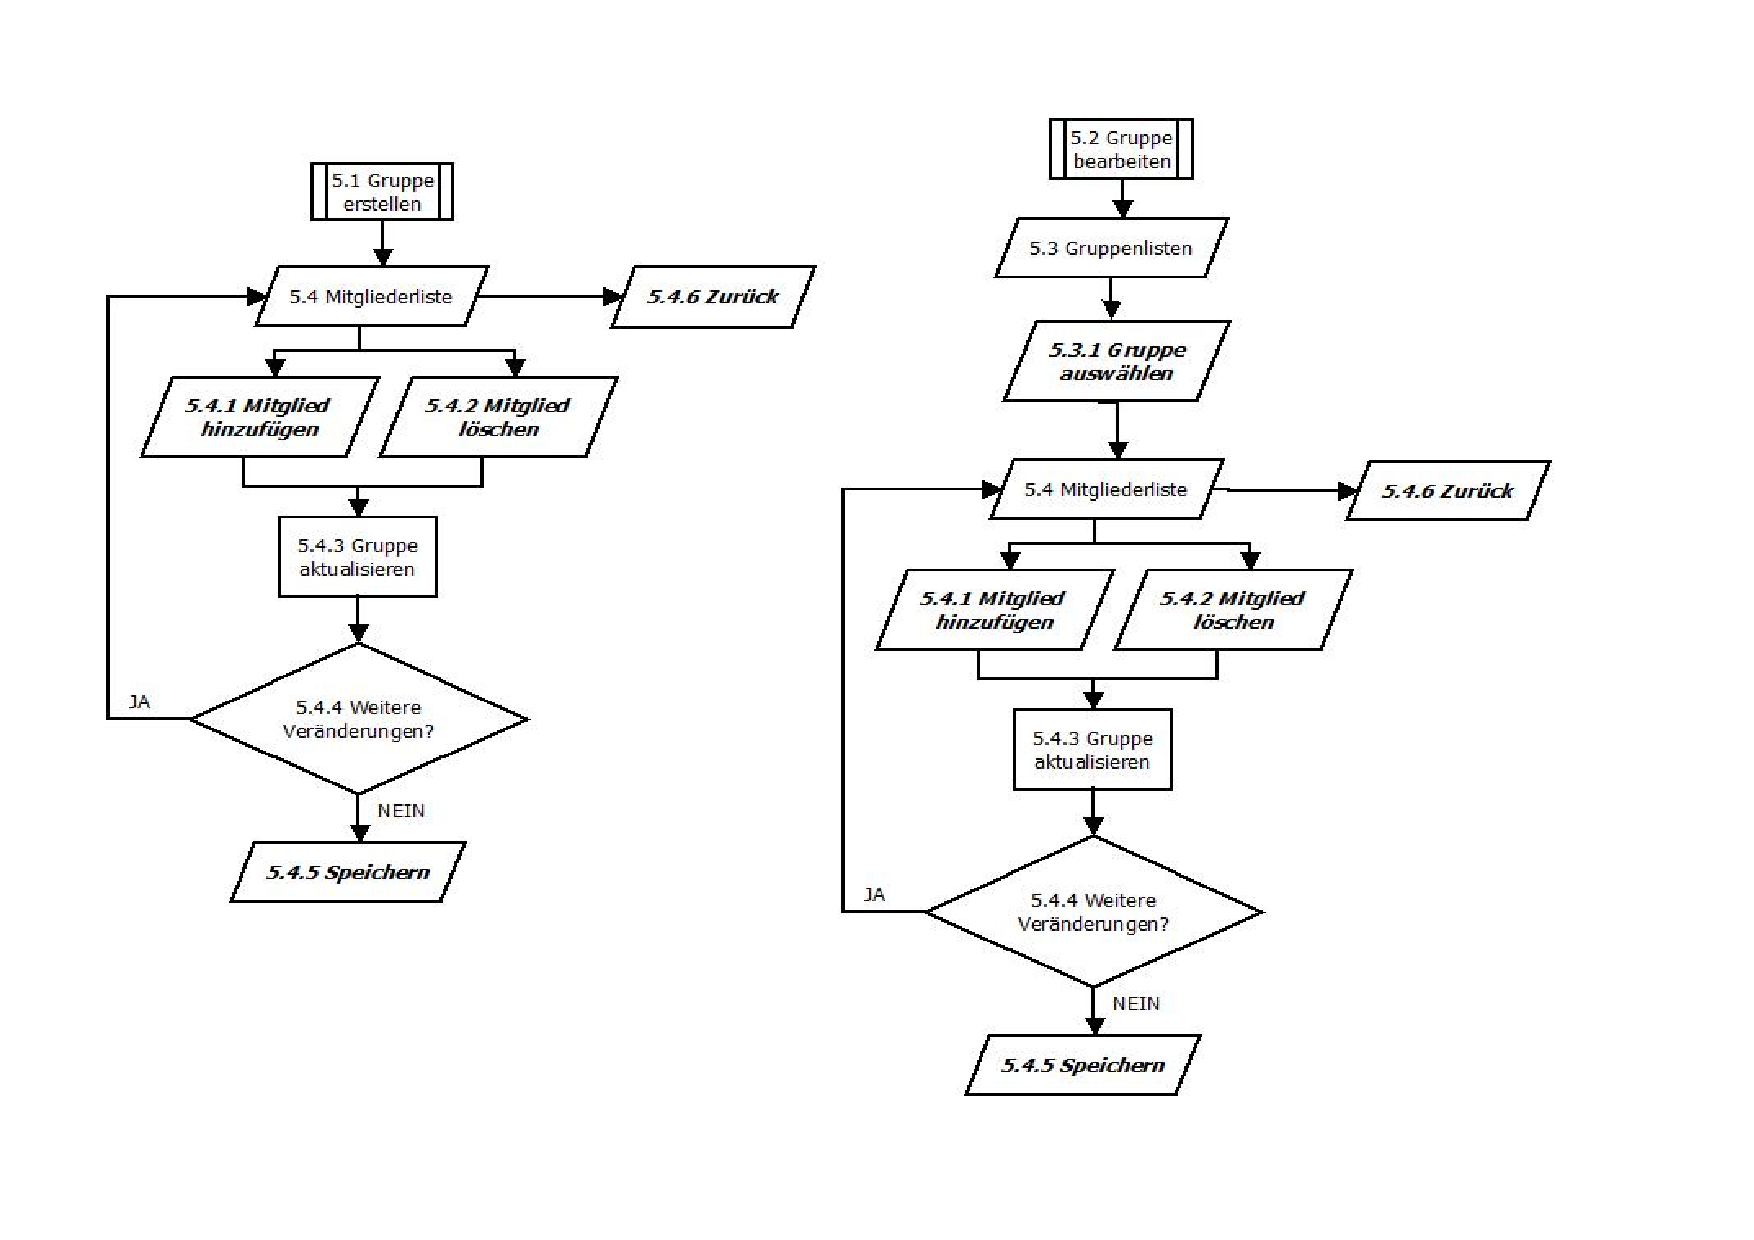
\includegraphics[trim=10mm 20mm 0mm 20mm,clip, scale=0.7]{Gruppenverwaltung.pdf}
\\
\footnotesize Abbildung 9: Gruppenverwaltung
\normalsize
\newline
\newline
Die Gruppenverwaltung wird in zwei Teile unterteilt. Der Erste beschreibt die Gruppenerstellung. Wie im Flussdiagramm zu sehen, kann eine Gruppe angelegt werden, indem zunächst der Nutzer die Menüoption Mitgliederliste wählt und hier eine Gruppe erstellt. Dabei können Mitglieder hinzugefügt bzw. auch gelöscht werden.
\subsubsection*{Entwicklung}
Die Entwicklung hat lediglich den Teil der eigentlichen Gruppenerstellung integriert. Der Nutzer legt einen Gruppennamen fest und kann daraufhin die registrierten Nutzer hinzufügen und ggf. wieder entfernen. Ist die Gruppe erstellt, kann gespeichert werden.
Diese kann im Nachhinein noch nicht geändert werden, weil die Gruppe nicht angezeigt wird. Dies ist ein Problem, welches die Entwickler noch ausbessern werden.
%\newpage
\subsection{Auswertung}
Der Nutzer hat die Möglichkeit vergangene Einkäufe auswerten zu lassen. Es gibt die zeitliche Eingrenzung und eine Gruppenmitgliedereingrenzung, bei der alle vergangenen Einkäufe von bestimmten Gruppen zusammengefasst werden.
\\
\\
\hspace*{-10mm} 
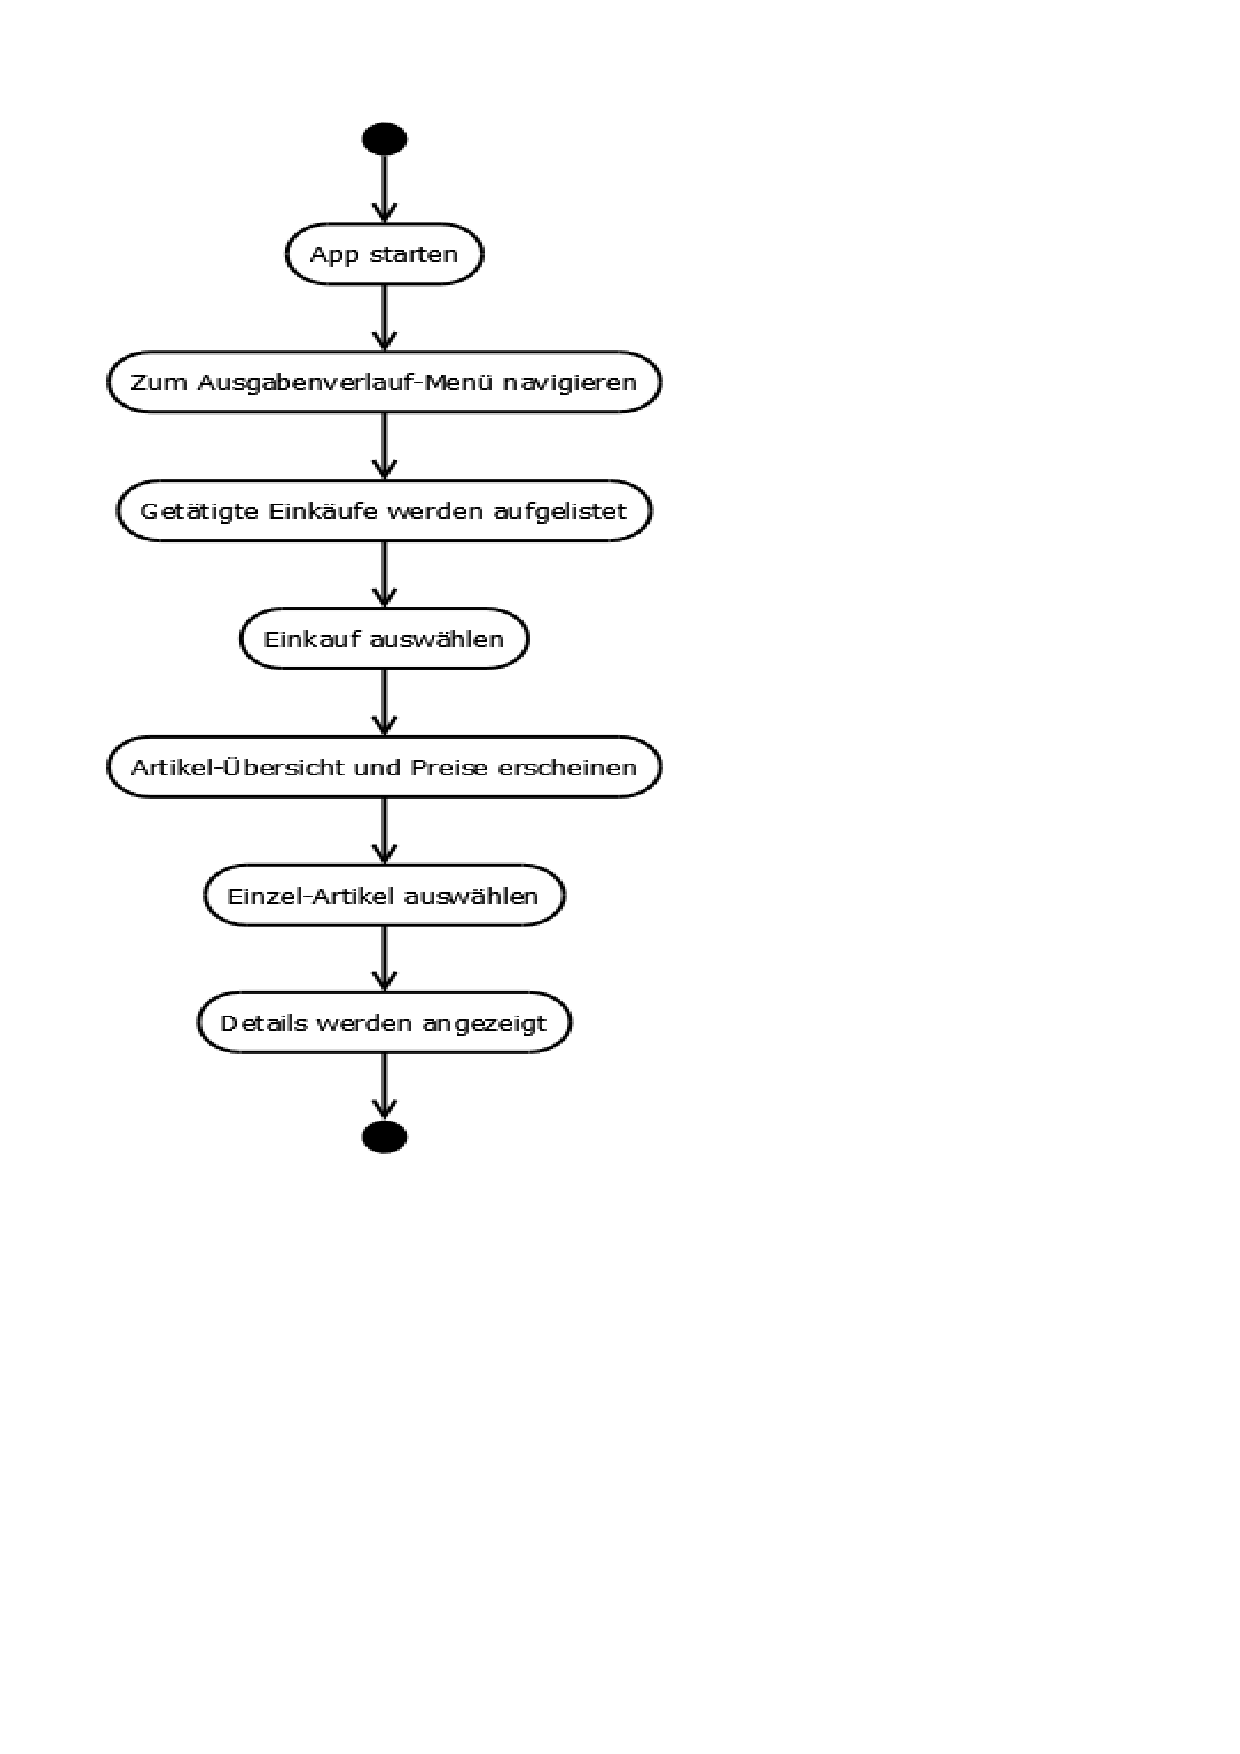
\includegraphics[trim = 17mm 130mm 0mm 20mm, clip, scale=0.9]{Aktiv-Ausgabe.pdf}
\\
\\
\footnotesize Abbildung 10: Aktivitätsdiagramm-Ausgabenverlauf
\normalsize
\\
\\
%\newpage
\subsubsection*{Zustandsdiagramm}
 „Ausgabenverlauf anzeigen“
\\
\\
\hspace*{-10mm} 
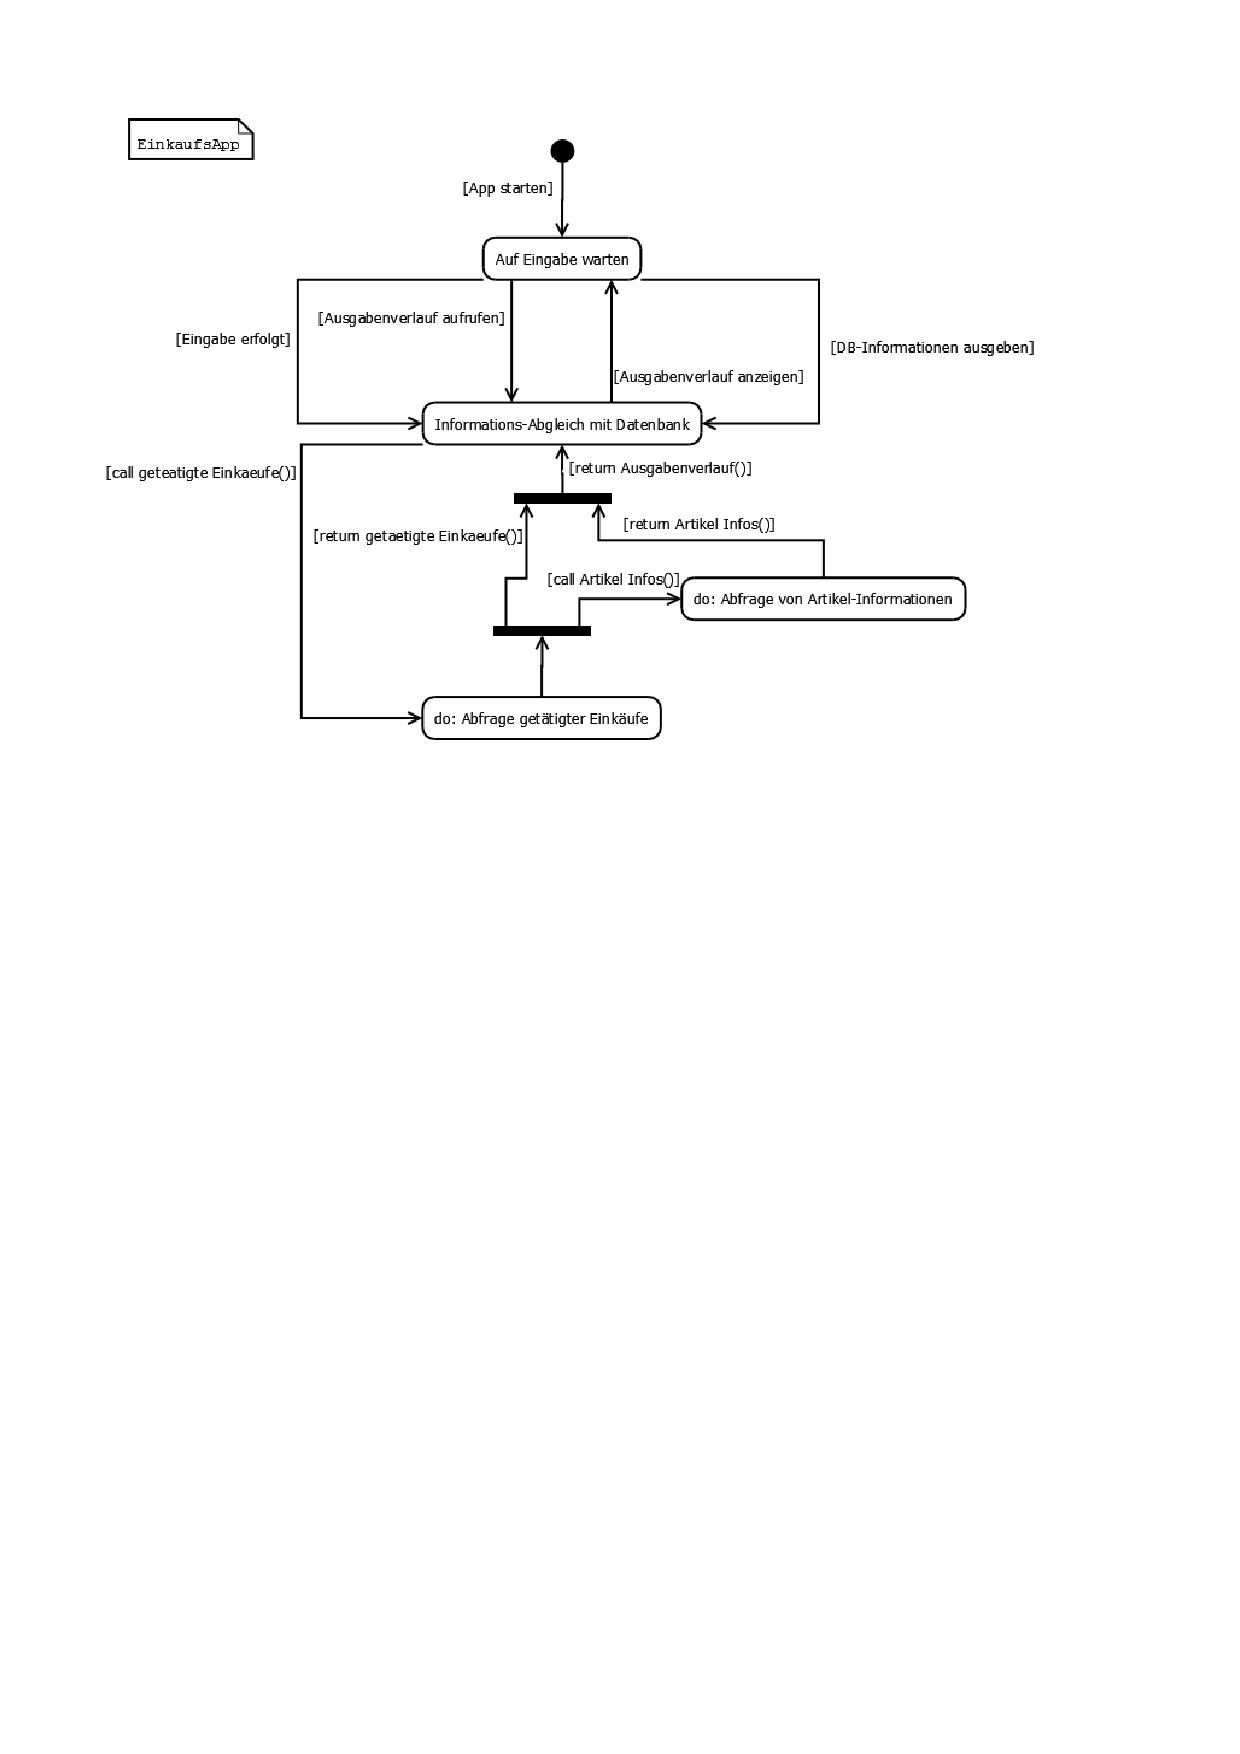
\includegraphics[trim = 17mm 130mm 0mm 20mm,clip]{Zustand.pdf}
\footnotesize Abbildung 9: Zustandsdiagramm
\normalsize
\subsubsection*{Design}
\hspace*{-10mm} 
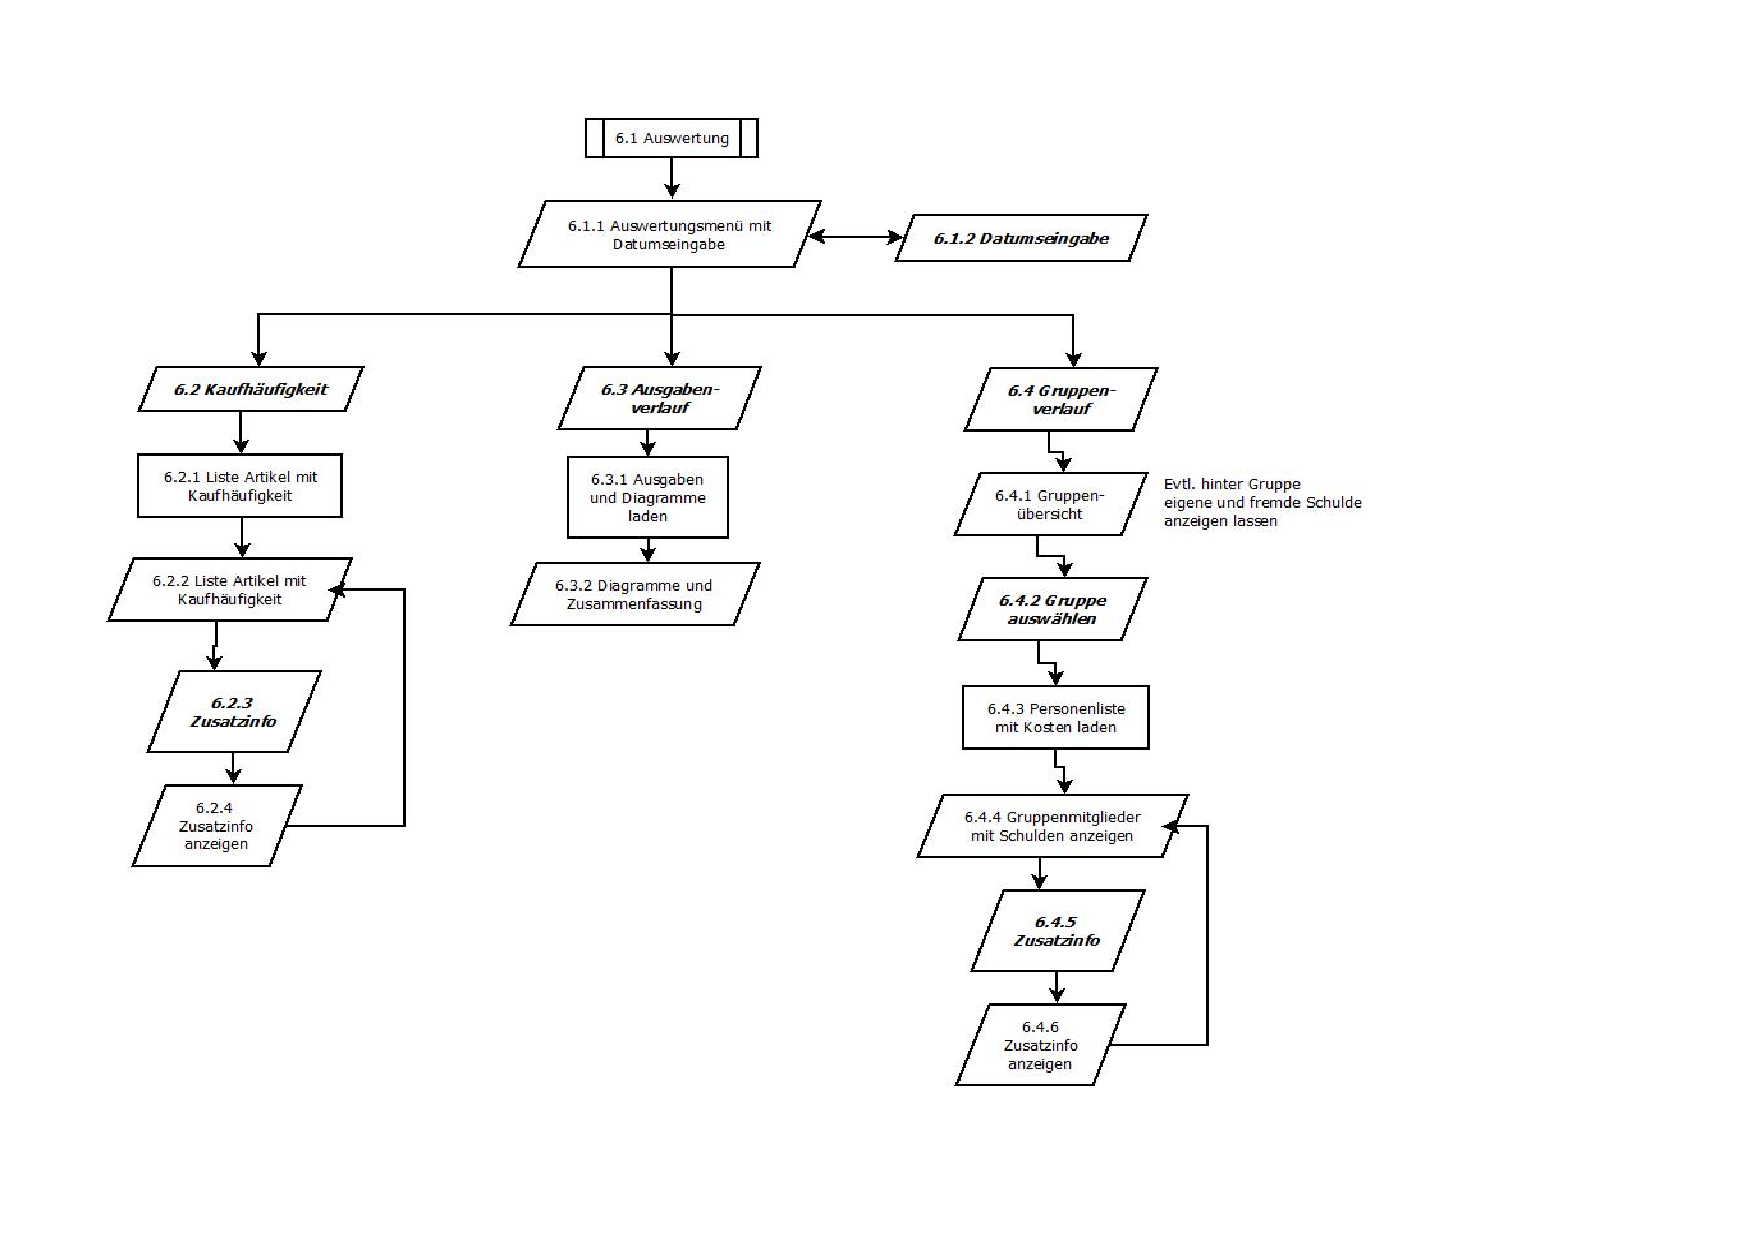
\includegraphics[trim = 20mm 60mm 0mm 20mm,clip,scale=0.9]{Auswertung.pdf}
\footnotesize Tabelle 4: Auswertung
\normalsize
\\
\subsubsection*{Auswertung der Diagramme}
In diesem Abschnitt wird noch einmal genauer auf die UML-Diagramme\footnote{Die gesamten UML-Diagramme befinden sich in dem Anhang der Dokumentation und werden vereinzelt in den Unterkapiteln schon dargestellt.} eingegangen, welche mit dem Enterprise Architect erstellt wurden. Der Enterprise Architekt eignet sich besonders gut zum Modellieren des Softwaresystems, da das Programm nach UML Standards arbeitet. Diese Funktionalität war besonders hilfreich beim Erstellen der UML-Diagramme. 
\\
Zudem bietet das Tool Vorlagen und Objekte für viele verschiedenen UML-Diagramme an und ist einfach zu bedienen. Gerade bei der ersten Erstellung eines UML-Diagramms bietet das Programm viele Hilfestellungen und ist optimal auf die Erstellung solcher Diagramme ausgelegt. Außerdem ist das Programm für den Anwender individuell anpassbar, um auch speziellen Anforderungen gerecht zu werden.
%\newpage
In der nachfolgenden Tabelle sind die Eigenschaften der in dem Projekt  genutzten Diagramme beschrieben und gegenübergestellt:
\\
\\
\hspace*{-10mm} 
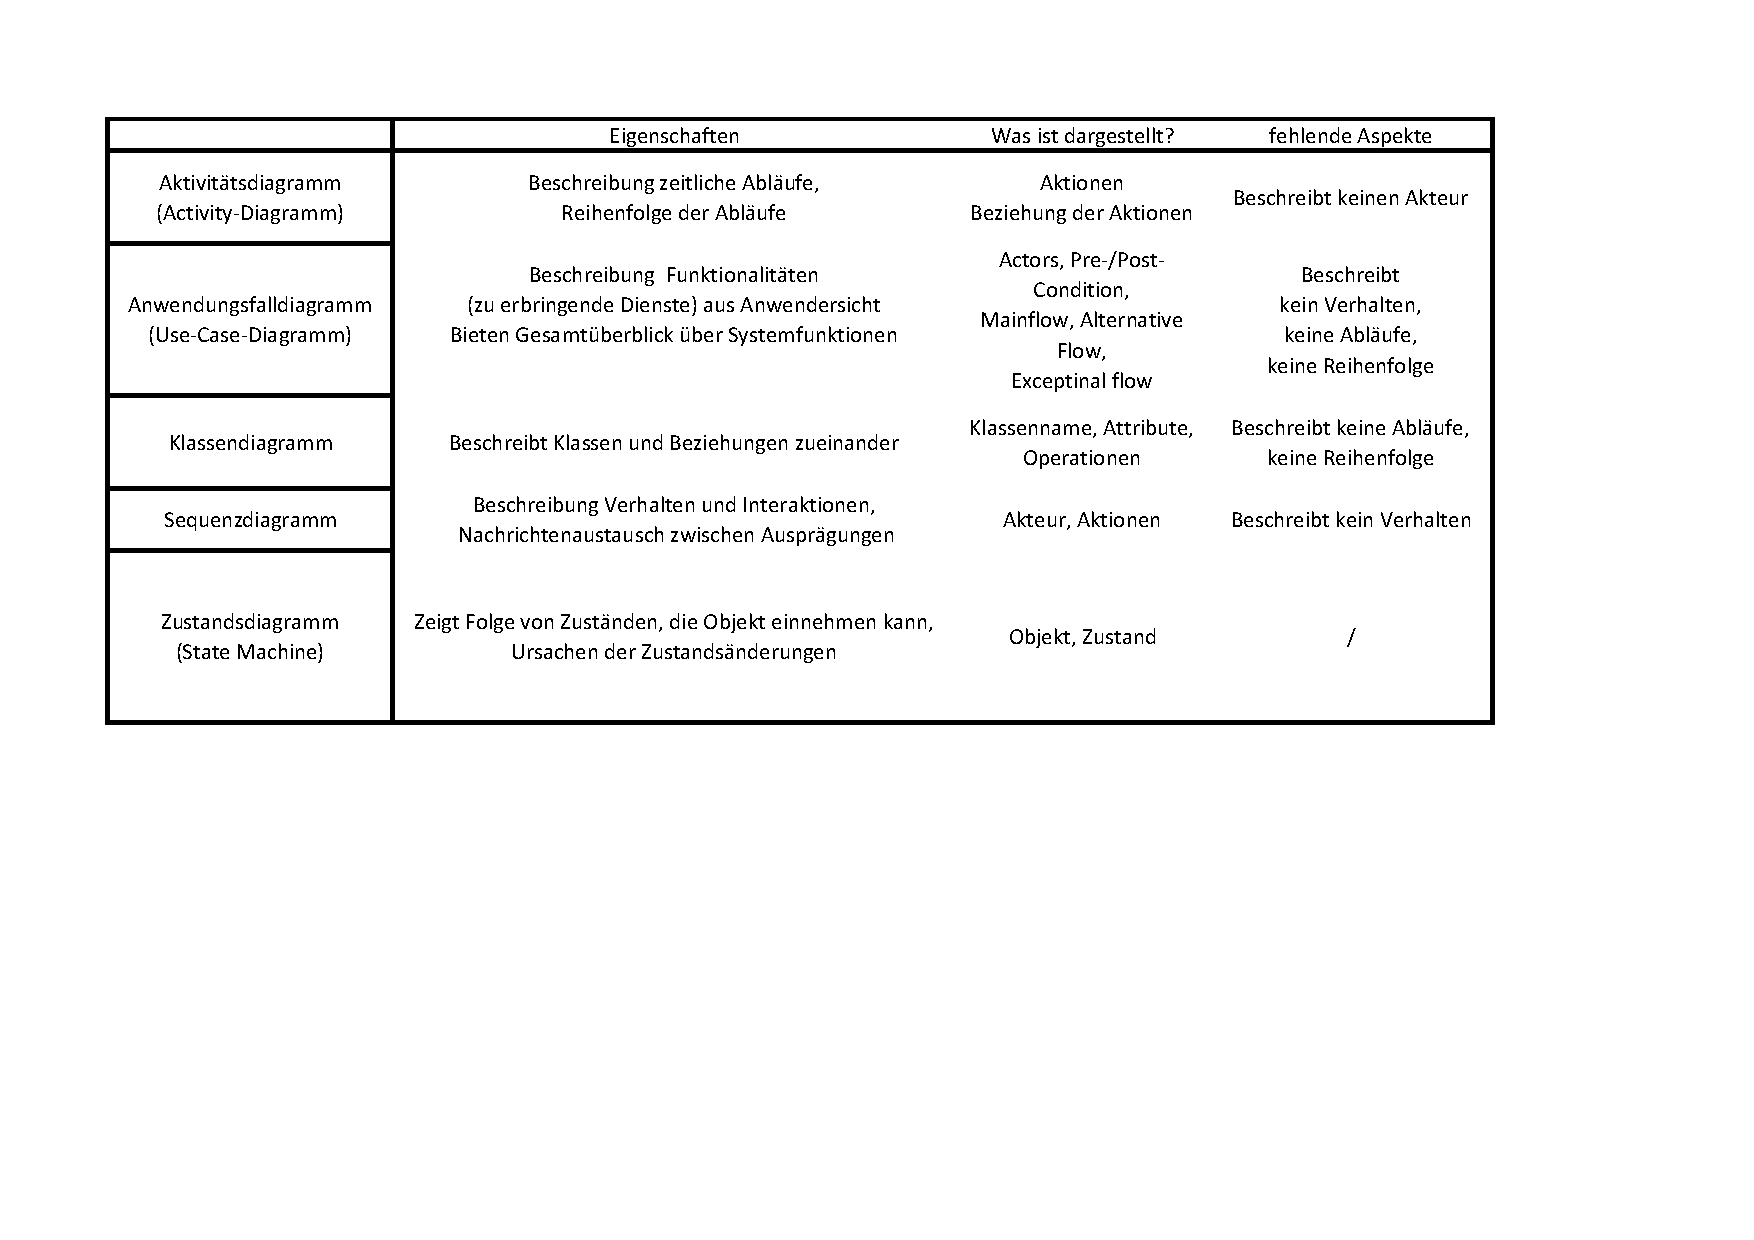
\includegraphics[trim = 10mm 60mm 0mm 20mm,clip,scale=0.7]{Auswertung_Diagramme.pdf}
\footnotesize Tabelle 4: Auswertung-Diagramme
\normalsize
\\
\\
Das Sequenzdiagramm muss innerhalb des Designprozesses konkretisiert dargestellt werden, damit die Entwickler optimal implementieren können.


\subsubsection*{Entwicklung}
%MH: Update von Eric einholen
%TO DO - HD: Eric nochmal anschreiben, wie es jetzt genau stant ist
%HD - 22.12.2015 Ja es wurde was umgesetzt. Ich weiß nur nicht, wie ich hierzu eine Text formulieren soll, der nicht wie Handbuch klingt
Wie im Programmablaufplan beschrieben, gibt es im View „Auswertung“ die drei Optionen Kaufhäufigkeit, Ausgabenverlauf und Gruppenverlauf. 
\\
\\
\textit{Kaufhäufigkeit}
\\
Die Funktionalität für diese Auswertung ist im Controller „PurchaseQuantityCtrl“ hinterlegt. Zuerst wird der Username abgefragt und es werden alle für die Auswertung relevanten Variablen auf 0 gesetzt. Anschließend wird ein Array mit den Artikeln angelegt und es wird nach der Kaufhäufigkeit sortiert. Es wird geprüft ob die UserID gleich der EinkaufsID ist und ob die Einkäufe im Zeitraum liegen. Wenn ja wird „Anzahl Einkäufe“ inkrementiert. Der gesamte Einkauf wird durchlaufen und die Gesamtausgaben aufaddiert. Falls ein Artikel schon im Array ist, wird die Gesamtanzahl aufgerechnet. Wenn alle Artikel erfasst sind werden dann die Preise ausgerechnet, gerundet und ausgegeben.
\\
\\
\textit {Ausgabenverlauf}
\\
Hierfür wird der Controller „PurchaseTimelineCtrl“ gebraucht. Darin werden zuerst die Daten festgelegt und der Username abgefragt. Anschließend werden alle Einkäufe nach Datum sortiert sodass der älteste Einkauf zuerst im Array steht. Wenn der User auch der Einkaufsowner ist und der Einkauf im angegebenen Zeitraum liegt, wird ein neues Label erstellt. Der Tagespreis wird auf 0 gesetzt. Anschließend werden alle Artikel des Einkaufes durchlaufen und die Gesamtkosten aufaddiert. Die Gesamtkosten sind dann der Datenpunkt. Zuletzt werden die Daten dann an „charData“ übergeben und ein Diagramm erstellt.
\\
\\
\textit {Gruppenverlauf}
\\
Es wird der Controller „GroupPurchase-TimelineCtrl“ verwendet. Auch hier wird zuerst der Username abgefragt. Es wird geprüft, ob ein Label schon vorhanden ist. Wenn das nicht der Fall ist, wird dieses als Datum hinzugefügt. Nach diesem Lauf sind alle Einkaufsdaten erfasst. Nun wird mit „SelectionSort“ sortiert. Wie bei der Kaufhäufigkeits-Auswertung werden auch hier alle Einkäufe durchlaufen. Für jedes Label wird ein Datenpunkt angegeben. Alle Artikel für jeden Einkauf werden erfasst, daraufhin wird der Gesamtpreis ermittelt. Es wird die richtige Stelle im Array gesucht, welche von Gruppe und Datum abhängt. Nachdem alle Datenpunkte angegeben wurden ist das Array komplett. Auch hier wird zuletzt alles an „chart.js“ übergeben und ein Diagramm wird erstellt.

%In jedem dieser Optionen muss ein Start- und Enddatum vom Nutzer festgelegt werden. Je nachdem welche Option ausgewählt wurde, sind die vom System gebende Informationen unterschiedlich. Da es aber weiterhin noch Probleme mit dem Einkaufsprozess gibt, kann die Auswertungsfunktion noch nicht genutzt werden.
%HD- Optionen werden am 24.12.15 eingefügt
\newpage
\section{Problemzusammenfassung}
%Hier wird das Ergebnis beschrieben.
\subsection{Usability der App}
Zusammengefasst kann die Version 1.0 der EinkaufsApp Nutzer registrieren und anmelden, sowie den Einkaufsprozess durchführen. Außerdem können Gruppen erstellt und verwaltet werden. Der Auswertungsprozess wurde in Anbetracht der Zeit nicht umgesetzt. Hinsichtlich der Optik wurde kein Corporate Design verwendet, um die Benutzerfreundlichkeit dennoch zu gewährleisten, implementierten die Entwickler ein übersichtliches Interface im aktuellen Web Stil.
%\newpage
\subsection{Besondere Herausforderungen des Projektes}
%\subsection{Organisation und Projektmanagement}
%MH: der Inhalt beist sich etwas mit der überschrift - lasst uns noch was besseres finden
Allem voran muss erwähnt werden, dass dieses Projekt enorm zeitkritisch war und daher die Planungsphase nahe zu vollständig übersprungen werden musste. Ebenfalls sind Design und Implementation stark parallelisiert abgelaufen. Um innerhalb von zwei Monaten ein lauffähiges und qualitätsorientiertes Software-Produkt zu erstellen, bedarf es eines überschaubaren und für alle Mitglieder transparenten Projektes, aber allem voran auch ein, gezielt auf die Herausforderungen, zugeschnittenes Team, welches die benötigten Skills und das Know-How bereits mitbringt. Ebenfalls ist es sehr wertvoll, wenn die Beteiligten bereits zuvor zusammen gearbeitet haben und untereinander mit Tools und Konventionen vertraut sind, oder zumindest in der Lage sind unter formalen Bedingungen zu arbeiten. Da naturgemäß in unserem Umfeld diese Voraussetzungen nur zu sehr geringen Teilen erfüllt werden können, ist auch ein sehr kritischer Projektablauf unausweichlich. Um diesen Schwierigkeiten entgegen zu wirken, wäre eine klarer Abgrenzung von Aufgabenbereichen
und Skills und auch das Vertrauen in diese Entscheidungen notwendig gewesen. Unglücklicherweise fehlte auch hier wieder die bereits erwähnte Planungsphase, die aber auch aus Zeit- und Lokalitätsgründen nicht umsetzbar war. Im weiteren Verlauf wurde dann eine zusätzliche Organisationseinheit zwischen dem Gesamtprojekt und den einzelnen Entwicklern eingefügt, um einen besseren Überblick zu gewährleisten und schneller Entscheidungen treffen zu können. An dieser Stelle lässt sich auch die obligatorische Diffizilität, die aus den unterschiedlichen Engagements entsteht erwähnen. Nach den vorangegangenen Ausführungen zu den kritischen Komponenten des Projektes sollte selbstredend sein, dass es ohne überdurchschnittlichen Einsatz jedes einzelnen Beteiligten
unmöglich zu 100\% in gegebener Zeit mit derartig begrenzten Ressourcen abgeschlossen werden kann. Nun sind naturgemäß die intrinsischen Beweggründe, sowie die Möglichkeiten der einzelnen Personen verschieden. Somit verbleibt die Aufgabe aller Beteiligten im Rahmen der gegebenen
Bedingungen das bestmöglich Ergebnis zu erzielen.
\newpage
\section{Projektabschluss}
\subsection{Aussichten}
In der folgenden Tabelle ist als kleine Übersicht gezeigt, welche Anforderungen an die EinkaufsApp umgesetzt wurden und welche noch nicht: 
\\
\\
\hspace*{-10mm} 
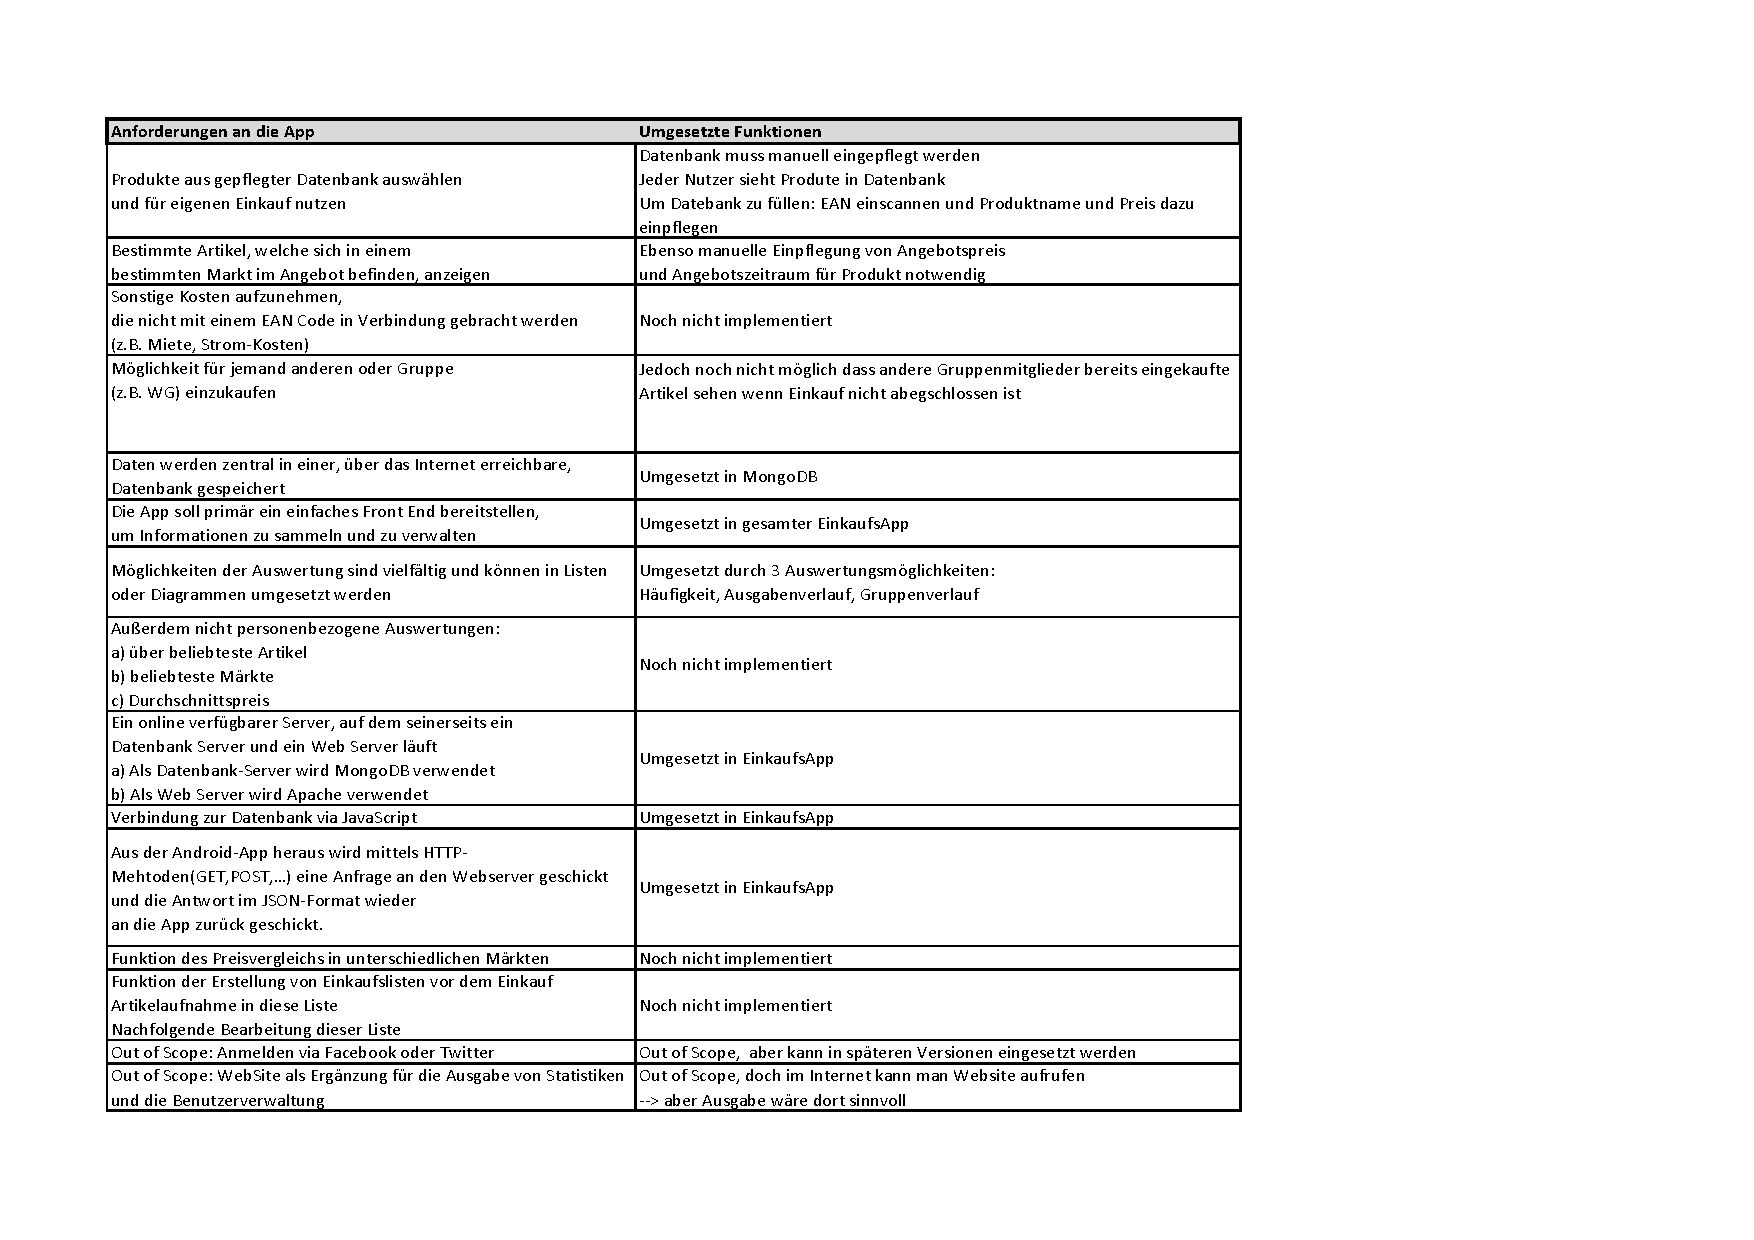
\includegraphics[trim = 17mm 10mm 0mm 20mm,clip,scale=0.9]{Anforderungen-Probleme.pdf}
\\
\footnotesize Tabelle 5: Aussichten
\normalsize
%\newpage
\subsection{Lesson learned}
%TO DO - MH (fazit)
Rückblickend war es eine besondere Herausforderung die gleiche Vorstellung der Aufgaben und Ziele im gesamten Team zu erreichen. Hierfür sind interne Abstimmungen innerhalb des Teams noch vor dem Projektstart sehr zu empfehlen. Ebenso ist eine im Vorfeld gut geplante und abgestimmte Organisationsstruktur unerlässlich. Da diese Vorarbeit hier nicht gegeben werden konnte, wurde zuerst auf eine Flache Hierarchie mit einem hohen Teil an Selbstorganisation für jede Person gesetzt. Dies hatte das Ziel jede Person mit einem signifikanten Maß an Verantwortung und Einsicht in die Sie umgebenden Projektgeschehnisse zu versehen, um die Qualität der geleisteten Arbeit zu sichern. Leider haben die Vorteile einer unkomplizierten und schnellen Kommunikation, sowie das flexible Arbeiten hier nicht überwogen. Demzufolge wurde eine weitere Organisationsebene über den Teilbereich ''Entwicklung'' eingefügt. Nachdem hier, abgetrennt von den anderen Arbeitsgruppen, kleinere Arbeitspakete erstellt wurden, ist die Produktivität spürbar gestiegen. \\
Weiterhin ist für das Arbeiten miteinander und das Verständnis der Ergebnisse ein gewisses Anteil an formalen Methoden sehr zu empfehlen. Es wurde vor allem in der Anfangsphase des Projektes relativ viel Zeit damit verbracht, sich über die Arbeitsmittel, das Vorgehen in den einzelnen Gruppen, die Ziele in den Gruppen und innerhalb des gesamten Projektes, sowie die Nachhaltigkeit und den Nutzen der verrichteten Arbeiten einig zu werden. Diese Herausforderung wäre ebenfalls bereits in der Planungsphase zu bewältigen.\\
Als ein weiteren sehr wichtigen Erfolgsfaktor ist das eigene Team und jedes Einzelne seiner Mitglieder als Stakeholder, zu betrachten. Hier können die Relevanz einzelner Personen für den Projekterfolg oder auch Ihre Motivation diesbezüglich stark variieren. Im Idealfall wird das Team, wie bereits zuvor bei den besonderen Herausforderungen erwähnt, konkret auf die spezifischen auftreten Aufgaben zugeschnitten und dann im vollen Umfang mit einer qualitativ hochwertigen Lösung betraut.\\
Ebenfalls ist in diesem Projekt Zeit eine sehr Herausfordernde Komponente gewesen. Da hier ein fixer Abgabetermin unausweichlich ist und darüber hinaus alle Mitglieder nicht Vollzeit an diesem Projekt arbeiten, wirken Abwesenheiten der einzelnen Personen besonders schwer. Da dieses Risiko aber unabdingbar ist, kann es lediglich in der Planung berücksichtigt werden.\\
+Somit sind die kritischsten Punkte, die in einem Softwareprojekt wie diesem beachten werden sollten, eine klare Definition der Aufgaben unter Berücksichtigung der zu Verfügung stehenden Zeit und der Personenressource, sowie ihrer Ausfallwahrscheinlichkeit. Allerdings auch die Zusammenstellung des Teams bezogen auf Motivation und Skills und nicht zuletzt eine ausreichende Planung des gesamten Projektes mit allen beteiligten, um die Erwartungen und die notwendigen Arbeiten klar abzugrenzen, zu kommunizieren und auch entgegen zu nehmen.
\newpage
\section*{Quellen}
\addcontentsline{toc}{section}{Quellen}
\subsection*{Internetquellen}
\begin{itemize}
\item[1.]Ionic Framework: \url{http://ionicframework.com/}
\item[2.]Ionic Guide: \url{http://ionicframework.com/docs/guide/}
\item[3.]Ionic Getting Started: \url{http://ionicframework.com/getting-started/}
\item[4.]ngCordova - Plugin Seite \url{http://ngcordova.com/}
\item[5.]BarCode Scanner : Plugin \url{hhttp://ngcordova.com/docs/plugins/barcodeScanner/}
\item[6.]Beispiel Projekt: \url{https://github.com/bastisk/suedm}
\item[7.]Editor: \url{http://brackets.io/}
\item[8.]Angular JS-Kurs: \url{https://www.codeschool.com/courses/shaping-up-with-angular-js/}
\item[9.]Tutorial zum Routing: \url{https://scotch.io/tutorials/angular-routing-using-ui-router}
\item[10.]App-Projekt: \url{http://www.mobile2b.de/ablauf-app-projekt/}
\item[11.] Dokumentationshilfe: \url{http://www.tellsbells.de/dokuwebsite/tbdokumentation.pdf}
\item[12.] Dokumentationshilfe: \url{https://www.lecturio.de/magazin/projekte-dokumentieren/}
\item[13.] Open Source mit API über eine einfachen HTTP-GET-Reguest: \url{http://www.opengtindb.org/api.php}
\item[14.] Suchmaschine der Firma die GTIN-Nummern verwaltet: \url{http://www.gepir.de/v31/V31_client/gtin.aspx}
\end{itemize}
\newpage
\section*{Organisationstools}
\begin{itemize}
\item[-]Zentrale Ablage: GitHub
\item[-]Diskussionsrunden: Slack
\item[-]Informationsaustausch: via Email
\item[-]Diagramme darstellen: via Dia 
\item[-]Kreieren von Web-Prototypen: proto.io
\item[-]Datenbanken und Datenbankenverwaltung: MongoDB, RoboMongo
\end{itemize}
\newpage
\section*{Anhang}
\addcontentsline{toc}{section}{Anhang}
\begin{itemize}
\item Anhang [01]: Pflichtenheft
\item Anhang [02]: Handbuch
\item Anhang [03]: Installationsanleitung
\item Anhang [04]: Angebot
\item Anhang [05]: Proto.io Design
\item Anhang [06]: Prototyp
\item Anhang [07]: Datenfluss-PAP-EinkaufsApp
\item Anhang [08]: Klassendiagramm
\item Anhang [09]: MongoDB-Klassendiagramm
\item Anhang [10]: Factories
\item Anhang [11]: Aktivitätsdiagramm Ausgabenverlauf
\item Anhang [12]: Aktivitätsdiagramm Einkauf 
\item Anhang [13]: Anwendungsfalldiagramm  Ausgabenverlauf
\item Anhang [14]: Anwendungsfalldiagramm Einkauf 
\item Anhang [15]: Sequenzdiagramm Ausgabenverlauf
\item Anhang [16]: Sequenzdiagramm Einkauf
\item Anhang [17]: Zustandsdiagramm 



%HD: ich hoffe, dass ich nichts vergessen habe

%1worldsync --> gs1 

\end{itemize}
\end{document}

    Status API Training Shop Blog About Pricing 

    © 2015 GitHub, Inc. Terms Privacy Security Contact Help 


